\documentclass[a4paper]{article}
\setlength{\parskip}{2mm}
\usepackage{ifthen}
\usepackage{amssymb}
\usepackage{multicol}
\usepackage{graphicx}
\usepackage[absolute]{textpos}
\usepackage{amsmath, amscd, amssymb, amsthm, latexsym}
% \usepackage[noload]{qtree}
%\usepackage{xspace,rotating,calligra,dsfont,ifthen}
\usepackage{xspace,rotating,dsfont,ifthen}
\usepackage[utf8]{inputenc}
\usepackage{pgfpages}
\usepackage{pgf,pgfarrows,pgfnodes,pgfautomata,pgfheaps,xspace,dsfont}
\usepackage{listings}
\usepackage{multicol}
\usepackage{todonotes}
\usepackage{url}
\usepackage{float}
\usepackage{framed,mdframed}
\usepackage{cancel}

\usepackage[strict]{changepage}


\makeatletter


\newcommand\hfrac[2]{\genfrac{}{}{0pt}{}{#1}{#2}} %\hfrac{}{} es un \frac sin la linea del medio

\newcommand\Wider[2][3em]{% \Wider[3em]{} reduce los m\'argenes
\makebox[\linewidth][c]{%
  \begin{minipage}{\dimexpr\textwidth+#1\relax}
  \raggedright#2
  \end{minipage}%
  }%
}


\@ifclassloaded{beamer}{%
  \newcommand{\tocarEspacios}{%
    \addtolength{\leftskip}{4em}%
    \addtolength{\parindent}{-3em}%
  }%
}
{%
  \usepackage[top=1cm,bottom=2cm,left=1cm,right=1cm]{geometry}%
  \usepackage{color}%
  \newcommand{\tocarEspacios}{%
    \addtolength{\leftskip}{3em}%
    \setlength{\parindent}{0em}%
  }%
}

\newcommand{\encabezadoDeProc}[4]{%
  % Ponemos la palabrita problema en tt
%  \noindent%
  {\normalfont\bfseries\ttfamily proc}%
  % Ponemos el nombre del problema
  \ %
  {\normalfont\ttfamily #2}%
  \
  % Ponemos los parametros
  (#3)%
  \ifthenelse{\equal{#4}{}}{}{%
  \ =\ %
  % Ponemos el nombre del resultado
  {\normalfont\ttfamily #1}%
  % Por ultimo, va el tipo del resultado
  \ : #4}
}

\newcommand{\encabezadoDeTipo}[2]{%
  % Ponemos la palabrita tipo en tt
  {\normalfont\bfseries\ttfamily tipo}%
  % Ponemos el nombre del tipo
  \ %
  {\normalfont\ttfamily #2}%
  \ifthenelse{\equal{#1}{}}{}{$\langle$#1$\rangle$}
}

% Primero definiciones de cosas al estilo title, author, date

\def\materia#1{\gdef\@materia{#1}}
\def\@materia{No especifi\'o la materia}
\def\lamateria{\@materia}

\def\cuatrimestre#1{\gdef\@cuatrimestre{#1}}
\def\@cuatrimestre{No especifi\'o el cuatrimestre}
\def\elcuatrimestre{\@cuatrimestre}

\def\anio#1{\gdef\@anio{#1}}
\def\@anio{No especifi\'o el anio}
\def\elanio{\@anio}

\def\fecha#1{\gdef\@fecha{#1}}
\def\@fecha{\today}
\def\lafecha{\@fecha}

\def\nombre#1{\gdef\@nombre{#1}}
\def\@nombre{No especific'o el nombre}
\def\elnombre{\@nombre}

\def\practicas#1{\gdef\@practica{#1}}
\def\@practica{No especifi\'o el n\'umero de pr\'actica}
\def\lapractica{\@practica}


% Esta macro convierte el numero de cuatrimestre a palabras
\newcommand{\cuatrimestreLindo}{
  \ifthenelse{\equal{\elcuatrimestre}{1}}
  {Primer cuatrimestre}
  {\ifthenelse{\equal{\elcuatrimestre}{2}}
  {Segundo cuatrimestre}
  {Verano}}
}


\newcommand{\depto}{{UBA -- Facultad de Ciencias Exactas y Naturales --
      Departamento de Computaci\'on}}

\newcommand{\titulopractica}{
  \centerline{\depto}
  \vspace{1ex}
  \centerline{{\Large\lamateria}}
  \vspace{0.5ex}
  \centerline{\cuatrimestreLindo de \elanio}
  \vspace{2ex}
  \centerline{{\huge Pr\'actica \lapractica -- \elnombre}}
  \vspace{5ex}
  \arreglarincisos
  \newcounter{ejercicio}
  \newenvironment{ejercicio}{\stepcounter{ejercicio}\textbf{Ejercicio
      \theejercicio}%
    \renewcommand\@currentlabel{\theejercicio}%
  }{\vspace{0.2cm}}
}


\newcommand{\titulotp}{
  \centerline{\depto}
  \vspace{1ex}
  \centerline{{\Large\lamateria}}
  \vspace{0.5ex}
  \centerline{\cuatrimestreLindo de \elanio}
  \vspace{0.5ex}
  \centerline{\lafecha}
  \vspace{2ex}
  \centerline{{\huge\elnombre}}
  \vspace{5ex}
}


%practicas
\newcommand{\practica}[2]{%
    \title{Pr\'actica #1 \\ #2}
    \author{Algoritmos y Estructuras de Datos I}
    \date{Primer Cuatrimestre 2022}

    \maketitlepractica{#1}{#2}
}

\newcommand \maketitlepractica[2] {%
\begin{center}
\begin{tabular}{r cr}
 \begin{tabular}{c}
{\large\bf\textsf{\ Algoritmos y Estructuras de Datos I\ }}\\
Primer Cuatrimestre 2022\\
\title{\normalsize Gu\'ia Pr\'actica #1 \\ \textbf{#2}}\\
\@title
\end{tabular} &
\begin{tabular}{@{} p{1.6cm} @{}}
\includegraphics[width=1.6cm]{logodpt.jpg}
\end{tabular} &
\begin{tabular}{l @{}}
 \emph{Departamento de Computaci\'on} \\
 \emph{Facultad de Ciencias Exactas y Naturales} \\
 \emph{Universidad de Buenos Aires} \\
\end{tabular}
\end{tabular}
\end{center}

\bigskip
}


% Símbolos varios

\newcommand{\nat}{\ensuremath{\mathds{N}}}
\newcommand{\ent}{\ensuremath{\mathds{Z}}}
\newcommand{\float}{\ensuremath{\mathds{R}}}
\newcommand{\bool}{\ensuremath{\mathsf{Bool}}}
\newcommand{\True}{\ensuremath{\mathrm{true}}}
\newcommand{\False}{\ensuremath{\mathrm{false}}}
\newcommand{\Then}{\ensuremath{\rightarrow}}
\newcommand{\Iff}{\ensuremath{\leftrightarrow}}
\newcommand{\implica}{\ensuremath{\longrightarrow}}
\newcommand{\IfThenElse}[3]{\ensuremath{\mathsf{if}\ #1\ \mathsf{then}\ #2\ \mathsf{else}\ #3\ \mathsf{fi}}}
\newcommand{\In}{\textsf{in }}
\newcommand{\Out}{\textsf{out }}
\newcommand{\Inout}{\textsf{inout }}
\newcommand{\yLuego}{\land _L}
\newcommand{\oLuego}{\lor _L}
\newcommand{\implicaLuego}{\implica _L}
\newcommand{\cuantificador}[5]{%
	\ensuremath{(#2 #3: #4)\ (%
		\ifthenelse{\equal{#1}{unalinea}}{
			#5
		}{
			$ % exiting math mode
			\begin{adjustwidth}{+2em}{}
			$#5$%
			\end{adjustwidth}%
			$ % entering math mode
		}
	)}
}

\newcommand{\existe}[4][]{%
	\cuantificador{#1}{\exists}{#2}{#3}{#4}
}
\newcommand{\paraTodo}[4][]{%
	\cuantificador{#1}{\forall}{#2}{#3}{#4}
}

% Símbolo para marcar los ejercicios importantes (estrellita)
\newcommand\importante{\raisebox{0.5pt}{\ensuremath{\bigstar}}}


\newcommand{\rango}[2]{[#1\twodots#2]}
\newcommand{\comp}[2]{[\,#1\,|\,#2\,]}

\newcommand{\rangoac}[2]{(#1\twodots#2]}
\newcommand{\rangoca}[2]{[#1\twodots#2)}
\newcommand{\rangoaa}[2]{(#1\twodots#2)}

%ejercicios
\newtheorem{exercise}{Ejercicio}
\newenvironment{ejercicio}[1][]{\begin{exercise}#1\rm}{\end{exercise} \vspace{0.2cm}}
\newenvironment{items}{\begin{enumerate}[a)]}{\end{enumerate}}
\newenvironment{subitems}{\begin{enumerate}[i)]}{\end{enumerate}}
\newcommand{\sugerencia}[1]{\noindent \textbf{Sugerencia:} #1}

\lstnewenvironment{code}{
    \lstset{% general command to set parameter(s)
        language=C++, basicstyle=\small\ttfamily, keywordstyle=\slshape,
        emph=[1]{tipo,usa}, emphstyle={[1]\sffamily\bfseries},
        morekeywords={tint,forn,forsn},
        basewidth={0.47em,0.40em},
        columns=fixed, fontadjust, resetmargins, xrightmargin=5pt, xleftmargin=15pt,
        flexiblecolumns=false, tabsize=2, breaklines, breakatwhitespace=false, extendedchars=true,
        numbers=left, numberstyle=\tiny, stepnumber=1, numbersep=9pt,
        frame=l, framesep=3pt,
    }
   \csname lst@SetFirstLabel\endcsname}
  {\csname lst@SaveFirstLabel\endcsname}


%tipos basicos
\newcommand{\rea}{\ensuremath{\mathsf{Float}}}
\newcommand{\cha}{\ensuremath{\mathsf{Char}}}
\newcommand{\str}{\ensuremath{\mathsf{String}}}

\newcommand{\mcd}{\mathrm{mcd}}
\newcommand{\prm}[1]{\ensuremath{\mathsf{prm}(#1)}}
\newcommand{\sgd}[1]{\ensuremath{\mathsf{sgd}(#1)}}

\newcommand{\tuple}[2]{\ensuremath{#1 \times #2}}

%listas
\newcommand{\TLista}[1]{\ensuremath{seq \langle #1\rangle}}
\newcommand{\lvacia}{\ensuremath{[\ ]}}
\newcommand{\lv}{\ensuremath{[\ ]}}
\newcommand{\longitud}[1]{\ensuremath{|#1|}}
\newcommand{\cons}[1]{\ensuremath{\mathsf{addFirst}}(#1)}
\newcommand{\indice}[1]{\ensuremath{\mathsf{indice}}(#1)}
\newcommand{\conc}[1]{\ensuremath{\mathsf{concat}}(#1)}
\newcommand{\cab}[1]{\ensuremath{\mathsf{head}}(#1)}
\newcommand{\cola}[1]{\ensuremath{\mathsf{tail}}(#1)}
\newcommand{\sub}[1]{\ensuremath{\mathsf{subseq}}(#1)}
\newcommand{\en}[1]{\ensuremath{\mathsf{en}}(#1)}
\newcommand{\cuenta}[2]{\mathsf{cuenta}\ensuremath{(#1, #2)}}
\newcommand{\suma}[1]{\mathsf{suma}(#1)}
\newcommand{\twodots}{\ensuremath{\mathrm{..}}}
\newcommand{\masmas}{\ensuremath{++}}
\newcommand{\matriz}[1]{\TLista{\TLista{#1}}}

\newcommand{\seqchar}{\TLista{\cha}}


% Acumulador
\newcommand{\acum}[1]{\ensuremath{\mathsf{acum}}(#1)}
\newcommand{\acumselec}[3]{\ensuremath{\mathrm{acum}(#1 |  #2, #3)}}

% \selector{variable}{dominio}
\newcommand{\selector}[2]{#1~\ensuremath{\leftarrow}~#2}
\newcommand{\selec}{\ensuremath{\leftarrow}}

\newcommand{\pred}[3]{%
    {\normalfont\bfseries\ttfamily\noindent pred }%
    {\normalfont\ttfamily #1}%
    \ifthenelse{\equal{#2}{}}{}{\ (#2) }%
    \{%
    \begin{adjustwidth}{+2em}{}
      \ensuremath{#3}
    \end{adjustwidth}
    \}%
    {\normalfont\bfseries\,\par}%
}

\newenvironment{proc}[4][res]{%

  % El parametro 1 (opcional) es el nombre del resultado
  % El parametro 2 es el nombre del problema
  % El parametro 3 son los parametros
  % El parametro 4 es el tipo del resultado
  % Preambulo del ambiente problema
  % Tenemos que definir los comandos requiere, asegura, modifica y aux
  \newcommand{\pre}[2][]{%
    {\normalfont\bfseries\ttfamily Pre}%
    \ifthenelse{\equal{##1}{}}{}{\ {\normalfont\ttfamily ##1} :}\ %
    \{\ensuremath{##2}\}%
    {\normalfont\bfseries\,\par}%
  }
  \newcommand{\post}[2][]{%
    {\normalfont\bfseries\ttfamily Post}%
    \ifthenelse{\equal{##1}{}}{}{\ {\normalfont\ttfamily ##1} :}\
    \{\ensuremath{##2}\}%
    {\normalfont\bfseries\,\par}%
  }
  \renewcommand{\aux}[4]{%
    {\normalfont\bfseries\ttfamily aux\ }%
    {\normalfont\ttfamily ##1}%
    \ifthenelse{\equal{##2}{}}{}{\ (##2)}\ : ##3\, = \ensuremath{##4}%
    {\normalfont\bfseries\,;\par}%
  }
  \renewcommand{\pred}[3]{%
    {\normalfont\bfseries\ttfamily pred }%
    {\normalfont\ttfamily ##1}%
    \ifthenelse{\equal{##2}{}}{}{\ (##2) }%
    \{%
    \begin{adjustwidth}{+5em}{}
      \ensuremath{##3}
    \end{adjustwidth}
    \}%
    {\normalfont\bfseries\,\par}%
  }

  \newcommand{\res}{#1}
  \vspace{1ex}
  \noindent
  \encabezadoDeProc{#1}{#2}{#3}{#4}
  % Abrimos la llave
  \{\par%
  \tocarEspacios
}
% Ahora viene el cierre del ambiente problema
{
  % Cerramos la llave
  \noindent\}
  \vspace{1ex}
}


\newcommand{\aux}[4]{%
    {\normalfont\bfseries\ttfamily\noindent aux\ }%
    {\normalfont\ttfamily #1}%
    \ifthenelse{\equal{#2}{}}{}{\ (#2)}\ : #3\, = \ensuremath{#4}%
    {\normalfont\bfseries\,;\par}%
}


% \newcommand{\pre}[1]{\textsf{pre}\ensuremath{(#1)}}

\newcommand{\procnom}[1]{\textsf{#1}}
\newcommand{\procil}[3]{\textsf{proc #1}\ensuremath{(#2) = #3}}
\newcommand{\procilsinres}[2]{\textsf{proc #1}\ensuremath{(#2)}}
\newcommand{\preil}[2]{\textsf{Pre #1: }\ensuremath{#2}}
\newcommand{\postil}[2]{\textsf{Post #1: }\ensuremath{#2}}
\newcommand{\auxil}[2]{\textsf{fun }\ensuremath{#1 = #2}}
\newcommand{\auxilc}[4]{\textsf{fun }\ensuremath{#1( #2 ): #3 = #4}}
\newcommand{\auxnom}[1]{\textsf{fun }\ensuremath{#1}}
\newcommand{\auxpred}[3]{\textsf{pred }\ensuremath{#1( #2 ) \{ #3 \}}}

\newcommand{\comentario}[1]{{/*\ #1\ */}}

\newcommand{\nom}[1]{\ensuremath{\mathsf{#1}}}


% En las practicas/parciales usamos numeros arabigos para los ejercicios.
% Aca cambiamos los enumerate comunes para que usen letras y numeros
% romanos
\newcommand{\arreglarincisos}{%
  \renewcommand{\theenumi}{\alph{enumi}}
  \renewcommand{\theenumii}{\roman{enumii}}
  \renewcommand{\labelenumi}{\theenumi)}
  \renewcommand{\labelenumii}{\theenumii)}
}



%%%%%%%%%%%%%%%%%%%%%%%%%%%%%% PARCIAL %%%%%%%%%%%%%%%%%%%%%%%%
\let\@xa\expandafter
\newcommand{\tituloparcial}{\centerline{\depto -- \lamateria}
  \centerline{\elnombre -- \lafecha}%
  \setlength{\TPHorizModule}{10mm} % Fija las unidades de textpos
  \setlength{\TPVertModule}{\TPHorizModule} % Fija las unidades de
                                % textpos
  \arreglarincisos
  \newcounter{total}% Este contador va a guardar cuantos incisos hay
                    % en el parcial. Si un ejercicio no tiene incisos,
                    % cuenta como un inciso.
  \newcounter{contgrilla} % Para hacer ciclos
  \newcounter{columnainicial} % Se van a usar para los cline cuando un
  \newcounter{columnafinal}   % ejercicio tenga incisos.
  \newcommand{\primerafila}{}
  \newcommand{\segundafila}{}
  \newcommand{\rayitas}{} % Esto va a guardar los \cline de los
                          % ejercicios con incisos, asi queda mas bonito
  \newcommand{\anchodegrilla}{20} % Es para textpos
  \newcommand{\izquierda}{7} % Estos dos le dicen a textpos donde colocar
  \newcommand{\abajo}{2}     % la grilla
  \newcommand{\anchodecasilla}{0.4cm}
  \setcounter{columnainicial}{1}
  \setcounter{total}{0}
  \newcounter{ejercicio}
  \setcounter{ejercicio}{0}
  \renewenvironment{ejercicio}[1]
  {%
    \stepcounter{ejercicio}\textbf{\noindent Ejercicio \theejercicio. [##1
      puntos]}% Formato
    \renewcommand\@currentlabel{\theejercicio}% Esto es para las
                                % referencias
    \newcommand{\invariante}[2]{%
      {\normalfont\bfseries\ttfamily invariante}%
      \ ####1\hspace{1em}####2%
    }%
    \newcommand{\Proc}[5][result]{
      \encabezadoDeProc{####1}{####2}{####3}{####4}\hspace{1em}####5}%
  }% Aca se termina el principio del ejercicio
  {% Ahora viene el final
    % Esto suma la cantidad de incisos o 1 si no hubo ninguno
    \ifthenelse{\equal{\value{enumi}}{0}}
    {\addtocounter{total}{1}}
    {\addtocounter{total}{\value{enumi}}}
    \ifthenelse{\equal{\value{ejercicio}}{1}}{}
    {
      \g@addto@macro\primerafila{&} % Si no estoy en el primer ej.
      \g@addto@macro\segundafila{&}
    }
    \ifthenelse{\equal{\value{enumi}}{0}}
    {% No tiene incisos
      \g@addto@macro\primerafila{\multicolumn{1}{|c|}}
      \bgroup% avoid overwriting somebody else's value of \tmp@a
      \protected@edef\tmp@a{\theejercicio}% expand as far as we can
      \@xa\g@addto@macro\@xa\primerafila\@xa{\tmp@a}%
      \egroup% restore old value of \tmp@a, effect of \g@addto.. is

      \stepcounter{columnainicial}
    }
    {% Tiene incisos
      % Primero ponemos el encabezado
      \g@addto@macro\primerafila{\multicolumn}% Ahora el numero de items
      \bgroup% avoid overwriting somebody else's value of \tmp@a
      \protected@edef\tmp@a{\arabic{enumi}}% expand as far as we can
      \@xa\g@addto@macro\@xa\primerafila\@xa{\tmp@a}%
      \egroup% restore old value of \tmp@a, effect of \g@addto.. is
      % global
      % Ahora el formato
      \g@addto@macro\primerafila{{|c|}}%
      % Ahora el numero de ejercicio
      \bgroup% avoid overwriting somebody else's value of \tmp@a
      \protected@edef\tmp@a{\theejercicio}% expand as far as we can
      \@xa\g@addto@macro\@xa\primerafila\@xa{\tmp@a}%
      \egroup% restore old value of \tmp@a, effect of \g@addto.. is
      % global
      % Ahora armamos la segunda fila
      \g@addto@macro\segundafila{\multicolumn{1}{|c|}{a}}%
      \setcounter{contgrilla}{1}
      \whiledo{\value{contgrilla}<\value{enumi}}
      {%
        \stepcounter{contgrilla}
        \g@addto@macro\segundafila{&\multicolumn{1}{|c|}}
        \bgroup% avoid overwriting somebody else's value of \tmp@a
        \protected@edef\tmp@a{\alph{contgrilla}}% expand as far as we can
        \@xa\g@addto@macro\@xa\segundafila\@xa{\tmp@a}%
        \egroup% restore old value of \tmp@a, effect of \g@addto.. is
        % global
      }
      % Ahora armo las rayitas
      \setcounter{columnafinal}{\value{columnainicial}}
      \addtocounter{columnafinal}{-1}
      \addtocounter{columnafinal}{\value{enumi}}
      \bgroup% avoid overwriting somebody else's value of \tmp@a
      \protected@edef\tmp@a{\noexpand\cline{%
          \thecolumnainicial-\thecolumnafinal}}%
      \@xa\g@addto@macro\@xa\rayitas\@xa{\tmp@a}%
      \egroup% restore old value of \tmp@a, effect of \g@addto.. is
      \setcounter{columnainicial}{\value{columnafinal}}
      \stepcounter{columnainicial}
    }
    \setcounter{enumi}{0}%
    \vspace{0.2cm}%
  }%
  \newcommand{\tercerafila}{}
  \newcommand{\armartercerafila}{
    \setcounter{contgrilla}{1}
    \whiledo{\value{contgrilla}<\value{total}}
    {\stepcounter{contgrilla}\g@addto@macro\tercerafila{&}}
  }
  \newcommand{\grilla}{%
    \g@addto@macro\primerafila{&\textbf{TOTAL}}
    \g@addto@macro\segundafila{&}
    \g@addto@macro\tercerafila{&}
    \armartercerafila
    \ifthenelse{\equal{\value{total}}{\value{ejercicio}}}
    {% No hubo incisos
      \begin{textblock}{\anchodegrilla}(\izquierda,\abajo)
        \begin{tabular}{|*{\value{total}}{p{\anchodecasilla}|}c|}
          \hline
          \primerafila\\
          \hline
          \tercerafila\\
          \tercerafila\\
          \hline
        \end{tabular}
      \end{textblock}
    }
    {% Hubo incisos
      \begin{textblock}{\anchodegrilla}(\izquierda,\abajo)
        \begin{tabular}{|*{\value{total}}{p{\anchodecasilla}|}c|}
          \hline
          \primerafila\\
          \rayitas
          \segundafila\\
          \hline
          \tercerafila\\
          \tercerafila\\
          \hline
        \end{tabular}
      \end{textblock}
    }
  }%
  % \datosalumno
}

\newcommand{\datosalumno}{
  \vspace{0.4cm}
  \textbf{Apellidos:}

  \textbf{Nombres:}

  \textbf{LU:}

  \textbf{Correo electrónico:}

  \textbf{Nro. de carillas que adjunta:}
  \vspace{0.5cm}
}


% AMBIENTE CONSIGNAS
% Se usa en el TP para ir agregando las cosas que tienen que resolver
% los alumnos.
% Dentro del ambiente hay que usar \item para cada consigna

\newcounter{consigna}
\setcounter{consigna}{0}

\newenvironment{consignas}{%
  \newcommand{\consigna}{\stepcounter{consigna}\textbf{\theconsigna.}}%
  \renewcommand{\ejercicio}[1]{\item ##1 }
  \renewcommand{\proc}[5][result]{\item
    \encabezadoDeProc{##1}{##2}{##3}{##4}\hspace{1em}##5}%
  \newcommand{\invariante}[2]{\item%
    {\normalfont\bfseries\ttfamily invariante}%
    \ ##1\hspace{1em}##2%
  }
  \renewcommand{\aux}[4]{\item%
    {\normalfont\bfseries\ttfamily aux\ }%
    {\normalfont\ttfamily ##1}%
    \ifthenelse{\equal{##2}{}}{}{\ (##2)}\ : ##3 \hspace{1em}##4%
  }
  % Comienza la lista de consignas
  \begin{list}{\consigna}{%
      \setlength{\itemsep}{0.5em}%
      \setlength{\parsep}{0cm}%
    }
}%
{\end{list}}



% para decidir si usar && o ^
\newcommand{\y}[0]{\ensuremath{\land}}

% macros de correctitud
\newcommand{\semanticComment}[2]{#1 \ensuremath{#2};}
\newcommand{\namedSemanticComment}[3]{#1 #2: \ensuremath{#3};}


\newcommand{\local}[1]{\semanticComment{local}{#1}}

\newcommand{\vale}[1]{\semanticComment{vale}{#1}}
\newcommand{\valeN}[2]{\namedSemanticComment{vale}{#1}{#2}}
\newcommand{\impl}[1]{\semanticComment{implica}{#1}}
\newcommand{\implN}[2]{\namedSemanticComment{implica}{#1}{#2}}
\newcommand{\estado}[1]{\semanticComment{estado}{#1}}

\newcommand{\invarianteCN}[2]{\namedSemanticComment{invariante}{#1}{#2}}
\newcommand{\invarianteC}[1]{\semanticComment{invariante}{#1}}
\newcommand{\varianteCN}[2]{\namedSemanticComment{variante}{#1}{#2}}
\newcommand{\varianteC}[1]{\semanticComment{variante}{#1}}

\usepackage{lib/caratula} % Version modificada para usar las macros de algo1 de ~> https://github.com/bcardiff/dc-tex
\usepackage[spanish]{babel}
\usepackage{graphicx} % Required for inserting images
\usepackage{subfloat}
\usepackage{algpseudocode}
\usepackage{algorithm}
\usepackage[utf8]{inputenc} 
\usepackage{hyperref}
\usepackage{amsmath}
\usepackage{cite}
\usepackage{enumitem} %Roman enumerate item

\newcommand{\dato}{\textit{Dato}}
\newcommand{\individuo}{\textit{Individuo}}


\begin{document}

\materia{Métodos numéricos}
\submateria{Segundo Cuatrimestre de 2024}
\titulo{Trabajo Práctico 1 - Grupo 27 }
\subtitulo{Eliminación Gaussiana}


\integrante{Pérez Buitrago, Ailén}{180/17}{perezailen1997@gmail.com}
\integrante{Rivera, Christian}{184/15}{christiannahuelrivera@gmail.com}
\integrante{Visgarra, Matias}{567/11}{m.e.visgarra@outlook.com.ar}

\maketitle
\newpage

\tableofcontents
\newpage

% Sección para comentarios entre nosotros:
\iffalse
Para el ejercicio de los opcionales que nos piden creo que uno que puede no ser demasiado complejo y que se puede relacionar con la sección de error numérico es el punto 2. En el mismo habla de expandir la diagonalización para obtener la inversa de la matriz original. 
Acá se me ocurrio que se lo puede relacionar con el error numérico si a la inversa calculada por nosotros le hacemos el producto con la matriz original y obtenemos "matrices que son casi como identidad". Esto creo que puede estar bueno para la experimentación.

Cito el mail que nos mandó el profesor para explicar que con un solo ejercicio de los extra alcanza. "Buenas, este es un recordatorio para que incluyan ejercicios optativos. Recuerde qué como se había mencionado, la idea es que los que grupos con participantes que recursan la materia incluyan en el informe al menos un ejercicio optativo de los que figuran al final del enunciado. Puede ser cualquiera de los 3 que figuran. Cualquier cosa consultar.
"
\fi

\iffalse
PENDIENTES para reentrega:
- Arreglar diccionario del latex para que las letras con caracteres estén bien configuradas.
- arreglar los warnings / referencias (labels y refs) mal escritos.
- agregar experimento para el ejercicio opcional. Sobre precisión en la representación de los floats.
- expandir las conclusiones del trabajo (sección "conclusiones")
- Revisar que no faltan puntos del enunciado y luego eliminar títulos de las secciones que referencian a los puntos del enunciado (ejemplo ejercicio 2.3)
- expandir la intruducción teórica para "difusión" y "difusión 2d".
- para la sección 7.2, reescribir la imagen en escala log y con mayores tamaños de matrices.
- expandir la sección de "tiempo de computo".
\fi

% ENUNCIADO del trabajo práctico https://campus.exactas.uba.ar/pluginfile.php/571695/mod_resource/content/16/TP1_2C_2024.pdf

% PAUTAS de redacción del informe https://campus.exactas.uba.ar/pluginfile.php/571693/mod_resource/content/3/pautas.pdf

\section{Resumen}
El objetivo de este trabajo práctico es presentar la implementación como también experimentación de algoritmos de eliminación gaussiana, haciendo hincapié en matrices tridiagonales y su aplicación en problemas de difusión. 

En la sección de introducción teórica iniciamos con una descripción detallada del proceso de eliminación gaussiana, tanto en su forma básica como en versiones optimizadas mediante técnicas de pivoteo. Además, se explora cómo estas técnicas pueden ser aplicadas eficazmente en la resolución de sistemas tridiagonales, con especial atención a su uso en el modelado del operador Laplaciano discreto. En la sección de desarrollo expandiremos sobre el trabajo realizado en los conceptos presentados en la introducción. Finalmente, en las secciones subsiguientes exploraremos problemas de presición numérica, y presentaremos un ejemplo práctico de un proceso de difusión modelado mediante estos métodos.

\textbf{Palabras claves:} \textit{eliminación gaussiana, matriz tridiagonal, difusión, operador Laplaciano}

%\section{Introducción}
%En el presente trabajo exploraremos la resolución de sistemas lineales analizando su implementación y experimentación con algoritmos de eliminación gaussiana y el estudio en particular del caso de matrices tridiagonales y su aplicación en el modelado de un problema de difusión.
\section{Marco teórico}

\subsection{Eliminación Gaussiana}
\label{sec:gaussiana}

Los sistemas de ecuaciones lineales pueden ser representados en forma matricial como \textit{Ax=b}, donde A representa la matriz de los coeficientes que acompañan a cada una de las incógnitas, \textit{x} representa al vector de incógnitas y \textit{b} al vector de términos independientes. Para los sistemas cuadrados, donde hay misma cantidad de incógnitas que de ecuaciones, el método de eliminación Gaussiana busca darle valor a los coeficientes del vector de incógnitas y resolver el sistema lineal. El modelado de sistemas de ecuaciones con matrices se extiende a una amplia gama de disciplinas como los gráficos por computadora, las finanzas y las ingenierías, entre otras, las cuales no serían como las conocemos sin este objeto y las operaciones que podemos hacer con él. 

\begin{figure}[H]
    \centering
    \begin{minipage}{0.3\linewidth}
        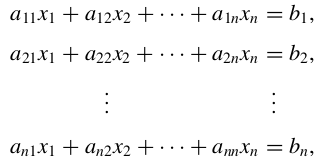
\includegraphics[width=\linewidth]{img/sistema_de_ecuaciones.png}
        \caption{Un sistema de ecuaciones}
    \end{minipage}
  \begin{minipage}{0.45\linewidth}
      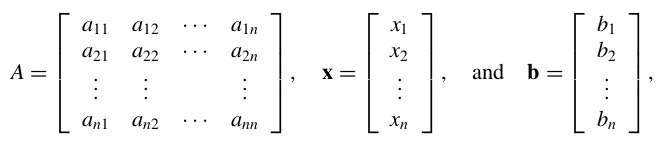
\includegraphics[width=\linewidth]{img/combinacion_lineal.png}
      \caption{Su forma matricial}
  \end{minipage}
  \caption{Sistemas de ecuaciones con su respectiva representación matricial}
\end{figure}

El proceso para resolver mediante este método comienza con la matriz original y se va aplicando sobre ella una serie de pasos hasta obtener una matriz de forma triangular superior. Para realizar esto, se recorre cada elemento $a_{ii}$ perteneciente a la diagonal principal, poniendo en ceros los elementos debajo de éste; este proceso se llama diagonalización. Una vez diagonalizado el sistema, buscamos darle valores a los coeficientes del vector de incógnitas por medio de un despeje desde abajo hacia arriba, es decir, empezamos por el coeficiente inferior del vector $x$ y subiendo por el mismo usando los valores despejados previamente para obtener nuevas soluciones para los próximos coeficientes. Éste  método descripto se conoce como \textit{Gaussian elimination with Backward substitution} \cite{Burden11}.
Considerando lo anterior, podemos notar que resolver el sistema de ecuaciones tiene una complejidad computacional de $\mathcal{O}(n^3)$.

\subsection{Métodos de pivoteo para diagonalización}
\label{sec:pivoteo}

Para casos donde encontramos, o  ``creamos'' por medio del mismo proceso de diagonalización, un cero en la diagonal de la matriz existen formas de obtener versiones equivalentes del sistema donde podemos continuar nuestro algoritmo de eliminación Gaussiana. Estos métodos se llaman \textit{pivoteos parciales o totales} y constan en hacer intercambios de filas o de columnas para que el sistema pueda seguir soportando el algoritmo. Cuando los intercambios son de filas los llamamos pivoteos parciales y cuando lo son de filas y columnas los llamamos pivotes totales. En el presente trabajo nos centraremos en pivoteos parciales. Observese en la figura \ref{fig:pivoting} como el proceso de eliminación gaussiana puede solucionar el hecho de encontrar un cero en la diagonal por medio del intercambio de filas.

\begin{figure}[H]
    $$
    \left[\begin{array}{cccc|c}
    2 & 2 & -1 & 3 & 13 \\
    -2 & -2 & 0 & 0 & -2 \\
    4 & -1 & -2 & 4 & 24 \\
    -6 & -2 & 2 & -3 & -10
    \end{array}\right] \rightarrow \begin{gathered}
    F_2-(-1) F_1 \\
    F_3-(2) F_1 \\
    F_4-(-3) F_1
    \end{gathered} \longrightarrow\left[\begin{array}{cccc|c}
    2 & 2 & -1 & 3 & 13 \\
    0 & \textbf{0} & -1 & 3 & 11 \\
    0 & -5 & 0 & -2 & -2 \\
    0 & 0 & -1 & 6 & 29
    \end{array}\right]\longrightarrow\left[\begin{array}{cccc|c}
    2 & 2 & -1 & 3 & 13 \\
    0 & -5 & 0 & -2 & -2 \\
    0 & 0 & -1 & 3 & 11 \\
    0 & 0 & -1 & 6 & 29
    \end{array}\right]
    $$
    
    \caption{El sistema de ecuaciones se encuentra con un cero en la diagonal luego del primer paso del algoritmo y debemos aplicar un intercambio entre la segunda y la tercer fila para poder continuar la diagonalización.}
    \label{fig:pivoting}

\end{figure}

\subsubsection{¿Todo sistema de ecuaciones se puede diagonalizar?}
\label{sec:sin_solucion}

Si una matriz es singular no tiene inversa. Esto ocurre cuando alguna fila de la matriz puede expresarse como combinación lineal de las otras filas. Por ejemplo, dada la siguiente matriz:

\begin{center}
$\begin{bmatrix}
1 & -1 & 3\\
-2 & 2 & -6\\
1 & 5 & 7
\end{bmatrix}$
\end{center}

La triangulación da como resultado la siguiente matriz:

\begin{center}
$\begin{bmatrix}
1 & 2 & 3\\
0 & 0 & 0\\
0 & 1 & 2
\end{bmatrix}$
\end{center}

Esta ecuación solo tiene resultado cuando b$_2$ es igual a 0. En ese caso tiene infinitas soluciones. Caso contrario, no existe solución.

Por este motivo no todo sistema de ecuaciones se puede diagonalizar más allá  del algoritmo que usemos.

\iffalse
Otro ejemplo, es tener una matriz tal que la primera columna tenga todos sus elementos iguales a 0. El problema aquí es que el primer elemento de la diagonal principal (posición [0,0]) es 0, lo que significa que no se puede usar como pivote.

\begin{center}
$\begin{bmatrix}
0 & 1 & -1 & 3\\
0 & -0.5 & 0 & 0\\
0 & 1 & -2 & 4\\
0 & -1 & 2 & -3
\end{bmatrix}$
\end{center}

\fi


\subsection{Matriz inversa: relaci´ón con la diagonalizaci´ón}
\label{opcionales}
\label{sec:inversa}

La matriz inversa de una matriz $A$, la cual denotaremos como $A^{-1}$, es una matriz que cumple con la propiedad de $A.A^{-1}=A^{-1}.A=I$ siendo $I$ la matriz identidad. Esta matriz inversa no siempre existe. Si la matriz $A$ cumple ser cuadrada y que su determinante \cite{Strang-determinante} sea distinto de cero, entonces esta matriz si existe.

Nuestro objetivo entonces, es calcular la matriz inversa de una matriz A utilizando el método de eliminación gaussiana (EG) con una matriz aumentada (figura \ref{fig:aumentada}). Este enfoque se basa en transformar la matriz A en su forma diagonal, y al mismo tiempo, aplicar las mismas operaciones a la matriz identidad para obtener la inversa de A.

El proceso consiste en construir una matriz aumentada que combine A y la matriz identidad I. Luego, mediante la eliminación gaussiana, se van realizando operaciones fila por fila para convertir A en la matriz identidad. Al final de este proceso, la matriz que acompaña a I será la inversa de A. Se puede ver un ejemplo de como se calcula la inversa en la figura (\ref{fig:jordan_ejemplo}). En la misma se puede apreciar cada paso como lo explicamos reci´én.

\begin{figure}[H]
    \centering
    \begin{minipage}{0.15\linewidth}
        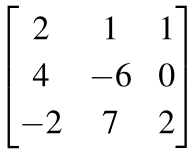
\includegraphics[width=\linewidth]{img/matriz-a-aumentar.png}
        \caption{Matriz A}
    \end{minipage}
  \begin{minipage}{0.3\linewidth}
      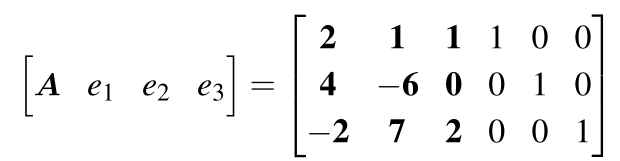
\includegraphics[width=\linewidth]{img/matriz-aumentada.png}
      \caption{Matriz ya aumentada}
  \end{minipage}
  \caption{Proceso de aumentar la matriz A.}
  \label{fig:aumentada}
\end{figure}

Este método es una aplicación práctica del algoritmo de Gauss-Jordan y es especialmente útil porque, a diferencia de otras técnicas, no requiere descomposición LU o factorizaciones complicadas. Lo que hacemos es simplemente aplicar operaciones de fila que son fáciles de implementar.

\begin{figure}[H]
    \centering
    \begin{minipage}{0.3\linewidth}
        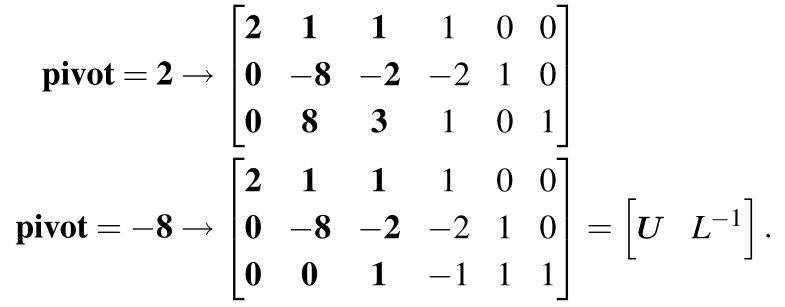
\includegraphics[width=\linewidth]{img/inversa_1.png}
        \caption{Triangular A}
    \end{minipage}
  \begin{minipage}{0.3\linewidth}
      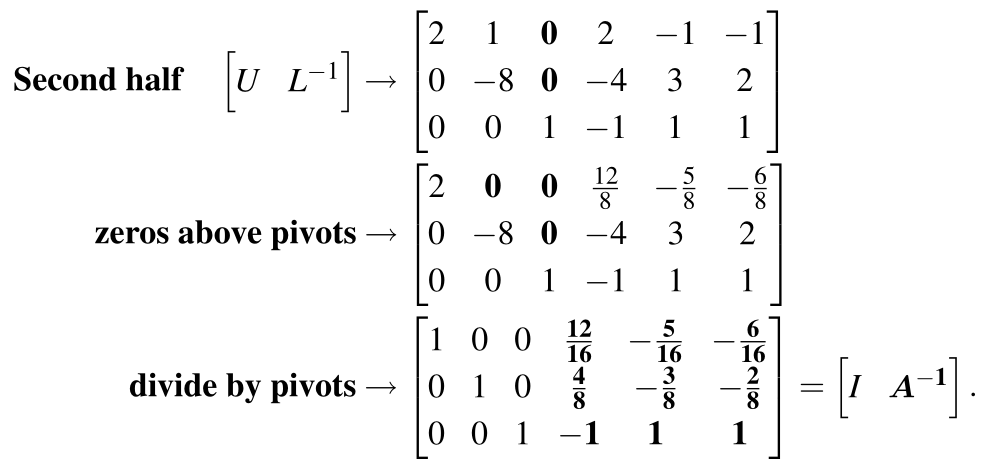
\includegraphics[width=\linewidth]{img/inversa_2.png}
      \caption{Convertir A en la identidad}
  \end{minipage}
  \caption{Ejemplo del algoritmo de Jordan para la matriz A.}
  \label{fig:jordan_ejemplo}
\end{figure}



\subsection{Sistemas tridiagonales}
\label{sec:tridiagonal}

Por su parte, las matrices tridiagonales, caracterizadas por su estructura rala, es decir, sus elementos son solo distintos de cero en la diagonal principal y en las diagonales adyacentes por encima y por debajo de esta, poseen propiedades que permiten operar con ellas con mayor eficiencia que con matrices genéricas. Para estos sistemas tridiagonales, se propone una implementación del algoritmo que reduce el número de operaciones aritméticas de $\mathcal{O}(n^3)$ a $\mathcal{O}(n)$. Esta optimización se consigue al aprovechar la estructura rala de la matriz, evitando cálculos redundantes sobre elementos nulos. Estos sistemas son estudiados en la bibliografía \cite{Recipes07} para dar soluciones eficientes al sistema tratando a cada una de las diagonales como vectores, como también a las incógnitas y a los términos independientes. Para comprender como es la estructura de los mismo puede ver en la figura \ref{fig:tridiagonal} donde logrará observar los vectores c, b, a, d y x los cuales son diagonal superior, diagonal principal, diagonal inferior, término independiente e incognitas respectivamente.  

\begin{figure}[h]

    \[ \begin{bmatrix}
b_1 & c_1 & & & 0\\
a_2 & b_2 & c_2 & & & \\
    & a_3 & b_3 & \ddots & \\
    &    & \ddots &  \ddots&c_{n-1}\\
0   &    &   & a_n & b_n
     \end{bmatrix}
  \begin{bmatrix}
        x_{1}\\
        x_{2} \\
        x_{3}\\ 
        \vdots\\ 
        x_{n}  
 \end{bmatrix}
 =
 \begin{bmatrix}
     d_{1} \\
     d_{2} \\
     d_{3} \\
     \vdots \\
     d_{n} \\
 \end{bmatrix}
 \]
 
 \caption{Estructura de un sistema tridiagonal.}
 \label{fig:tridiagonal}
\end{figure}

\subsection{Operador Laplaciano}
\label{Intro_laplaciano}
\label{sec:laplaciano}

El operador de Laplace o Laplaciano ($\nabla^{2}$) sobre funciones escalares es el diferencial para la divergencia del gradiente. Esto nos da una noción del comportamiento de la función que es utilizada para numerosos procesos físicos, como por ejemplo propagación de ondas o de calor \cite{laplaciano_web}. Este operador también lo podemos usar para problemas de difusión del estilo de caminatas aleatorias \cite{random_walk}

\subsection{Difusión}
\label{Intro_difusion}

 La difusión es un proceso estocástico cuyo modelado implica simular cómo una entidad, en este caso vista como calor, se distribuye en un medio. La ecuación de difusión, que describe este fenómeno, puede ser discretizada y resuelta mediante métodos numéricos. En particular, el operador Laplaciano (sic. \ref{sec:laplaciano}) es un operador diferencial que juega un papel central en la descripción de la difusión. En una dimensión, la versión discreta del Laplaciano es equivalente a la segunda derivada, y se utiliza en varias areas como en el procesamiento de imágenes y análisis de datos en redes.


\subsection{Operador Laplaciano 2D}
\label{Intro_laplaciano2D}
El operador laplaciano discreto en 2D es fundamental para modelar fenómenos como la difusión y el flujo de calor en una malla o grilla de puntos. Este operador se define generalmente como la suma de las diferencias de valores en los puntos vecinos, lo que permite calcular cómo cambia una cantidad en un punto respecto a sus alrededores.

\subsection{Difusión 2D}
\label{Intro_difusion2D}
 La difusión en dos dimensiones (2D) ofrece una perspectiva más compleja en comparación con la difusión unidimensional, ya que ésta permite modelar procesos como la propagación de calor, la dispersión de contaminantes y la dinámica de poblaciones. Utilizando el laplaciano discreto, vamos a establecer ecuaciones que simulan el proceso de difusión.
\section{Desarrollo}

En esta sección hablaremos en profundidad del \textbf{cómo} implementar los algorimos que presentamos en la sección anterior y los conceptos que hay que tener en cuenta si el lector los quiere implementar para sí.

\subsection{Desarrollo de los Algoritmos}

El lenguaje de programación utilizado para implementar los algoritmos fue Python. De esta forma, para representar a las matrices utilizamos la estructura de datos \textit{array[array[dtype='float32']]}. 
A su vez, se utilizo la librería Numpy para operaciones sobre matrices, el módulo Timeit para la medición de tiempos, y utilizamos Matplotlib para graficar los experimentos realizados.

Dejamos la el link a nuestra implementaci´ón \cite{Colab} para se pueda seguir la lectura del presente informe con un ejemplo real del c´ódigo. En el mismo se puede ver el c´ódigo fuente como tambi´én, testing y experimentaci´ón que profundizaremos en secciones proximas.

\subsection{Eliminación Gaussiana sin pivoteo}

Basado tanto en el pseudocódigo visto en la teórica \cite{teoEG} como en el libro \cite{Recipes07}, se implemento utilizando Python el algoritmo de eliminación Gausianna sin pivoteo. 
El siguiente pseudocódigo describe los pasos seguidos. Éste toma como input la matriz y el término independiente y devuelve la triangulación de la matriz input \textit{A} concatenada con el término independiente \textit{b}. Observemos también que se verifica que los elementos de la diagonal no queden nulos, si se diera el caso de esta situación se devuelve una excepción. (algoritmo \ref{EG_sinP})


\begin{algorithm}
\caption{Eliminación Gaussianna sin pivoteo}\label{EG_sinP}
\begin{algorithmic}
\State \textbf{EG}(\textbf{in} A : matrix,\textbf{in} b : vect) $\to \textbf{A}$
 
 \State $col \gets A.shape[1]$
 
 \For{$i \gets 0$ to $n-1$}
    \If{(equal$\_$zero($A[i][i]$))}
        \State  raise exception(‘‘Error, no se encuentra solución.'') 
    \EndIf

\For{$j \gets i+1$ to $n$}

    \State m$_{ij}$ = $\frac{a_{ji}}{a_{ii}}$
    
    \For{$k \gets i$ to col}
        \State a$_{jk}$ = a$_{jk}$ - $m_{ji}*{a_{ik}}$
    \EndFor

\EndFor
\EndFor
\end{algorithmic}
\end{algorithm}

De esta forma, la complejidad del algoritmo propuesto es $\mathcal{O}$(n$^3$) en el tamaño de la matriz.
Como mencionamos en la introducción teórica (sic \ref{sec:gaussiana}), una vez completada la eliminación hacia adelante, obtenemos una matriz triangular superior. Por lo tanto, podemos resolver el sistema de ecuaciones de manera directa utilizando \textit{backward substitution}, la cual implementamos de la siguiente manera llamando a la función \textit{resolver\_sistema} (algoritmo \ref{backwardSubst})

\begin{algorithm}
\caption{Backward Substitution}\label{backwardSubst}
\begin{algorithmic}
\State \textbf{resolver\_sistema}(\textbf{in} A : matrix, \textbf{in} b : vector) $\to \textbf{x}$
 \State A $\gets$ EG(A, b) 
\State n $\gets$ len(A)
\State x $\gets$ np.zeros(n)

\For{$i\gets n-1$ to $-1$ by $-1$}
    \State sum = 0
        
    \For{j $\gets$ $0$ to $n$ by $1$ }
        \If{i $!=$ j}
            \State sum $=$ sum $+ A[i][j] *$ x$[j]$
        \EndIf       
        \State x$[i]$ = $\frac{(A[i][n] - sum)}{A[i][i]}$
    \EndFor
\EndFor
\State \textbf{return $x$}
\end{algorithmic}
\end{algorithm}



\subsection{Eliminación Gaussiana con pivoteo} 
\label{seccion_EG_pivot}

La eliminación gaussiana con pivoteo parcial es una variante del algoritmo anterior que introdujimos en la secci´ón [\ref{sec:pivoteo}].
En este método, la elección del pivote para cada paso de eliminación hace que el algoritmo pueda resolver más problemas. El primer paso es buscar el elemento de mayor magnitud en la columna correspondiente, este elemento se intercambia con el elemento actual de la diagonal principal para garantizar que el pivote seleccionado tenga una magnitud relativamente grande, lo que reduce la posibilidad de errores numéricos debido a divisiones por valores cercanos a cero. 

\begin{algorithm}
\label{alg:pivoteo}
\caption{Eliminación Gaussiana con pivoteo}
\begin{algorithmic}[1]
\State \textbf{EG}(\textbf{in} A : matrix, \textbf{in} b : vector) $\to \textbf{A}$
 
 \State $col \gets A.shape[1]$
 
 \For{$i \gets 0$ to $n-1$}
    \If{(equal$\_$zero($A[i][i]$))}
        \State $max \gets i$
        \For{$j \gets i+1$ to $n-1$}
            \If{($A[j][i] != 0$ AND $(A[j][i]>A[max][i] or A[max][i]==0)$))}
                \State $max \gets j$
            \EndIf
        \EndFor
        \State $A[[i,max]] \gets A[[max,i]]$
    \EndIf
    \If{(equal$\_$zero($A[i][i]$))}
        \State  raise exception($"$Error, no se encuentra solución.$"$) 
    \EndIf
\EndFor
\For{$j \gets i+1$ to $n$}

    \State m$_{ij}$ = $\frac{a_{ji}}{a_{ii}}$
    
    \For{$k \gets i$ to col}
        \State a$_{jk}$ = a$_{jk}$ - $m_{ji}*{a_{ik}}$
    \EndFor

\EndFor
\end{algorithmic}
\end{algorithm}

En nuestro pseudoc´ódigo (algoritmo \ref{alg:pivoteo}) agregamos la l´ógica para buscar una fila que no tenga cero en nuestra columna y que adem´ás sea la de mayor magnitud a partir de la l´ínea 4 hasta la 11. C´ómo explicamos previamente en la secci´ón \ref{sec:sin_solucion}, puede no existir dicha posici´ón y de modo que a´ún as´í tenemos que confirmar que pudimos encontrar un intercambio, y sin´ó lanzar una excepci´ón.

\subsection{Eliminacion Gaussiana para sistemas tridiagonales}
\label{tridiagonal}
La eliminación gaussiana para sistemas tridiagonales es una adaptación eficiente de los algoritmos anteriores que aprovecha la estructura especial de las matrices tridiagonales. Estas matrices, como ya explicamos en la secci´ón [\ref{sec:tridiagonal}], tienen elementos distintos de cero solo en la diagonal principal y en las dos diagonales adyacentes a esta.
\begin{center}
    $a_{i}x_{i-1}+b_{i}x_{i}+c_{i}x_{i+1} = d_{i}$,
\end{center}
    
    

 Es así que para el caso de sistemas tridiagonales, el proceso de eliminación gaussiana se simplifica significativamente ya que la gran mayoría de sus elementos es cero, lo que permite reducir la cantidad de operaciones necesarias para triangular la matriz.
 
 Como nota interesante podemos decir que este algoritmo es un caso particular de algoritmos m´ás generales que resuelven los llamados \textbf{Band-Diagonal} \cite{Recipes07-Band} que tienen una estructura similar pero la cantidad de diagonales no nulas es mayor y adem´ás pueden no estar ubicadas de manera sim´étrica como en este caso. En otros libros se puede encontrar tambi´én un pseudoc´ódigo similar al que exploraremos aqu´í con el nombre de algoritmo de \textit{Thomas}. 

 %\subsubsection{Eliminación Gaussiana para sistemas tridiagonales sin precómputo}

 De las variantes que hay para este problema, la primer implementación es la estándar o sin precomputo. Este algoritmo resuelve en una única función el sistema Ax = b, sin necesidad de funciones auxiliares. El pseudocódigo que proponemos se puede ver en el algoritmo [\ref{alg:tridiagonal_simple}.

 \begin{algorithm}
 \label{alg:tridiagonal_simple}
\caption{EG para tridiagonales sin precómputo}
\begin{algorithmic}[1]
\State \textbf{tridiag}(\textbf{in} a : vector, \textbf{in} b : vector, \textbf{in} c : vector, \textbf{in} r : vector) $\to \textbf{u}$
\State n $\gets$ len(b)
\State u $\gets$ np.zeros(n)
\State gam $\gets$ np.zeros(n)
\State bet $\gets$ 0.0
\If{b[0] $==$ 0}
    \State \textbf{return} ``error: try another way''
\EndIf
\State u[0] $\gets$ r[0] / bet
\For{$j\gets 1$ to $n-1$}
    \State gam[j] $\gets$ c[j-1] / bet
    \State bet $\gets$ b[j] - (a[j-1] * gam[j])
    \If{bet $==$ 0.0}
        \State \textbf{return} ``error: try another way''
    \EndIf
    \State u[j] $\gets$ (r[j] - a[j-1] * u[j-1]) / bet
\EndFor
\For{$j\gets n-2$ to $0$}
    \State u[j] $\gets$ u[j] - gam[j+1] * u[j+1]
\EndFor
\State \textbf{return $u$}
\end{algorithmic}
\end{algorithm}

La ventaja de este algoritmo frente a Eliminación Gaussiana para matrices comunes es la reducción en la complejidad temporal y espacial. Más adelante se desarrolla sobre estos beneficios ( sección \ref{resultados}).



\subsubsection{Eliminación Gaussiana para sistemas tridiagonales con precómputo}

La segunda variante a implementar es aquella que utiliza precómputo. Este algoritmo resuelve el sistema $Ax = b$ en dos pasos. 
El primer paso se realiza de forma análoga a la triangulación de la matriz $A$, pero a nivel vectorial. De esta forma, debe modificar únicamente al vector $b$, ya que el vector $a$ debe ser cero después de la triangulación (por estar debajo de la diagonal) y el vector $c$ no se modifica en la triangulación. En forma paralela, debe precomputar cómo se debe modificar $d$ cuando efectivamente se pase como parámetro.

El siguiente paso es recibir el parámetro $d$ y ajustarlo según el precómputo. Luego, con el vector resultado del precómputo y el vector $c$ calculan el vector solución.

Sean \_gam y \_bet variables globales:

\begin{algorithm}[H]
\caption{EG para tridiagonales con precómputo}\label{tridiagonal_prec}
\begin{algorithmic}
\State \textbf{tridiagPrecomputo}(\textbf{in} a : vector, \textbf{in} b : vector, \textbf{in} c : vector, \textbf{in} r : vector) $\to \textbf{u}$
\State (gam,bet) $\gets$ tridiagAux(a,b,c)
\State u $\gets$ np.zeros(n)
\State u[0] $\gets$ r[0] / bet[0]
\For{$j \gets 1$ to $n-1$}
    \State u[j] $\gets$ (r[j] - a[j-1]*u[j-1]) / bet[j]
\EndFor
\For{$j \gets n-2$ to $0$}
    \State u[j] $\gets$ u[j] -  gam[j+1]*u[j+1]
\EndFor
\State \textbf{return} $u$
\end{algorithmic}
\end{algorithm}

\begin{algorithm}[H]
\caption{Función auxiliar para tridiagonales con precómputo}
\begin{algorithmic}
\State \textbf{tridiagAux}(\textbf{in} a : vector, \textbf{in} b : vector, \textbf{in} c : vector) $\to \textbf{(\_gam,\_bet)}$
\State n $\gets$ len(b)
\If{np.array\_equal(\_gam, np.zeros(n)) or np.array\_equal(\_bet, np.zeros(n))}
    \State \textbf{return} (\_gam,\_bet)
\EndIf
\State \_gam $\gets$ np.zeros(n)
\State \_bet $\gets$ np.zeros(n)
\If{b[0] $==$ 0}
    \State \textbf{return} ``error: try another way''
\EndIf
\State \_bet[0] $\gets$ b[0]
\For{$j \gets 1$ to $n-1$}
    \State \_gam[j] $\gets$ c[j-1] / \_bet[j-1]
    \State \_bet[j] $\gets$ b[j] - a[j-1] * \_gam[j]
    \If{\_bet[j] $==$ 0.0}
        \State \textbf{return} ``error: try another way''
    \EndIf
\EndFor
\State \textbf{return} (\_gam,\_bet)
\end{algorithmic}
\end{algorithm}

\subsection{Verificación de la implementación}
Para probar nuestra implementación de sistema tridiagonal se nos pidió resolver una serie de ecuaciones diferenciales. Debemos encontrar \textit{u} para el problema $\frac{\partial^2}{\partial x^2}u = d$ utilizando la matriz tridiagonal del operador laplaciano.
Como mencionamos anteriormente (sección \ref{Intro_laplaciano}), para el caso unidimensional la operación discreta de $\frac{\partial^2}{\partial x^2}u = d$ está dada por:

u$_{i-1}$ - 2u$_{i}$ + u$_{i+1}$ = d$_{i}$

Esta ecuación forma un sistema matricial como se muestra en la figura \ref{laplaciano}. Esta matriz es tridiagonal y siguiendo la estructura de la matriz de la sección \ref{tridiagonal} toma valores:

\begin{itemize}
    \item a: vector de valores 1.
    \item b: vector de valores -2.
    \item c: vector de valores 1.
\end{itemize}

\begin{figure}[H]
    \[ \begin{bmatrix}
-2 & 1 & & & 0\\
1 & -2 & 1 & & & \\
    & 1 & -2 & \ddots & \\
    &    & \ddots &  \ddots & 1\\
0   &    &   & 1 & -2
     \end{bmatrix}
     \begin{bmatrix}
           u_{1}\\
           u_{2} \\
           u_{3}\\ 
           \vdots\\ 
           u_{n}  
     \end{bmatrix}
      =
     \begin{bmatrix}
          d_{1} \\
          d_{2}\\
          d_{3}\\
         \vdots\\ 
         d_{n}  
     \end{bmatrix} \]
     \caption{Forma matricial}\label{laplaciano}
\end{figure}
Por esta estructura,  el algoritmo de eliminación gaussiana para tridiagonales puede aplicarse eficientemente resolviendo el sistema de ecuaciones resultantes de la discretización. Además, como la matriz es diagonal dominante, no es necesario el pivoteo pues no hay riesgo de división por cero. 

De esta forma, se modelaron los tres vectores $d$ a los cuales nombramos como d$\_vect\_a$, d$\_vec\_b$  y d$\_vec\_c$, que representan las ecuaciones requeridas que se pueden ver a continuación con parámetro $n=101$  y se calcularon las segundas derivadas para los tres casos utilizando el algoritmo que se encuentra en la sección \ref{tridiagonal}.

\begin{enumerate}[label=\alph*)] % (a), (b), (c), ...
\label{ec_ej4}
\item d$_{i}$ = 
    $\begin{cases}
      0\\
      \frac{4}{n} & i=\lfloor \frac{n}{2} \rfloor   +1
    \end{cases}$

\item d$_{i}$ = $\frac{4}{n^{2}}$

\item d$_{i}$ = $\frac{-1+2i}{(n-1)}\frac{12}{n^{2}}$

\end{enumerate}


Con estos resultados, se creó un único gráfico que se muestra en la siguiente Figura \ref{result_laplaciano} obteniendo el resultado esperado.

\begin{figure}[H]
\centerline{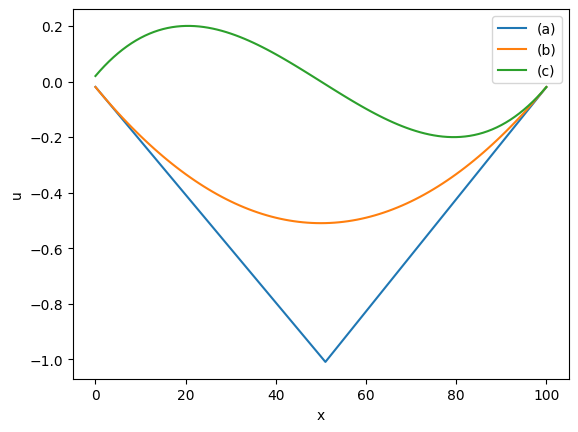
\includegraphics[scale=0.45]{./img/resultado_tridiag}}
\caption{Resultado de las funciones}
\label{result_laplaciano}
\end{figure}

Analizando con mayor profundidad cada función:\par
\begin{enumerate}
    \item[a)] La derivada segunda de la función (a) es 0 para todo x distinto a $i = n/2 + 1$. Luego, la derivada primera de la función (a) es constante para todo x $\not =$ i,lo que implica que la función es lineal para todo x $\not =$ i. Por lo que i es un punto de inflexión. Como la derivada segunda en i es positiva, la función tiene que ser cóncava para los positivos. Esta función descripta es coherente con la figura graficada.

    \item[b)] La derivada segunda de la función (b) es $\frac{4}{n^2}$ para todo x. Entonces, la derivada primera es lineal para todo x, lo que implica que la función es cuadrática para todo x. La función graficada se corresponde con una cuadrática.

    \item[c)] La derivada segunda de la función (c) es una función lineal para todo x. Esto significa que la derivada primera es cuadrática, implicando que la función debe ser un polinomio de grado tres (cúbica). La función graficada se corresponde con una cúbica.
\end{enumerate}



\subsection{Tiempos de cómputo}
Como explicamos anteriormente, los diferentes algoritmos tienen complejidades computacionales muy distintas, lo que afecta significativamente el tiempo de ejecución y los recursos necesarios para resolver un problema.

En el caso de la eliminación gaussiana, el algoritmo con pivoteo tiene una complejidad cúbica ($\mathcal{O}$(n$^3$)), lo que significa que el tiempo de ejecución crece rápidamente a medida que aumenta el tamaño de la matriz. Por otro lado, los algoritmos diseñados específicamente para matrices con estructura especial, como el caso de las matrices tridiagonales, pueden reducir esa complejidad a $\mathcal{O}$(n), lo que implica una mejora considerable en términos de rendimiento.Por lo tanto, Lo esperado es que el algoritmo tridiagonal sea notablemente más rápido a comparación del algoritmo de eliminación gaussiana con pivoteo

Para evaluar el rendimiento de los distintos algoritmos de eliminación gaussiana, se generaron matrices y vectores correspondientes a cada tamaño seleccionado. Posteriormente, se implementaron los algoritmos de eliminación gaussiana con pivoteo, eliminación gaussiana para matrices tridiagonales, tanto en su versión estándar como en la versión con precomputo, para dimensiones que corresponden a potencias de dos (2$^k$). Este proceso fue repetido 10 veces, registrando el tiempo mínimo de ejecución en cada iteración. Esta repetición busca mitigar el posible efecto de las variaciones causadas por la organización del computador (posición de las variables en memoria por ejemplo).

Considerando, las complejidades temporales teóricas de los algoritmos:

\begin{itemize}
    \item Eliminación Gaussiana con pivoteo: $O(n^{3})$
    \item Eliminación Gaussiana para matrices tridiagonales estándar: $O(n)$
    \item Eliminación Gaussiana para matrices tridiagonales con precomputo: $O(n)$
\end{itemize}


Definimos \textit{A} como la matriz Laplaciana, es decir, aquella matriz que tiene a -2 como elementos de la diagonal y a 1 como los elementos de las dos subdiagonales. Obtenemos el siguiente resultado (figura \ref{result_ej5})

\begin{figure}[H]
\centerline{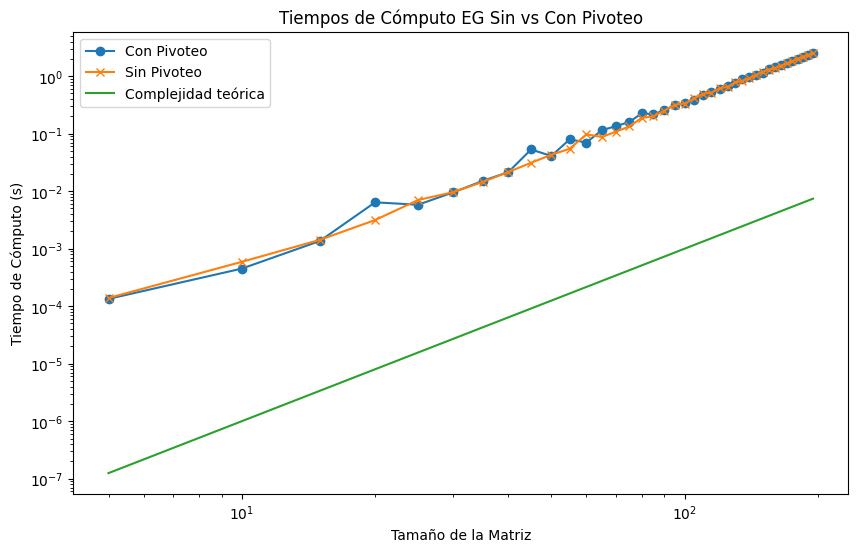
\includegraphics[scale=0.45]{./img/tiempos_EGsinVsConPivoteo.png}}
\caption{Tiempo de computo para EG con pivoteo y EG en un sistema tridiagonal}
\label{result_ej5}
\end{figure}

Como era esperado, como los algoritmos de las matrices tridiagonales trabajan a nivel vectorial, modificando los valores de los vectores b y c, la complejidad temporal mejora.

%Los resultados obtenidos se pueden ver en la sección \ref{resultados}


\subsection{Simulación de difusión}

Para expresar la ecuación de difusión se considera el incremento para el paso \textit{k}, $u^k - u^{k-1}$ como una
fracción ($\alpha$) del operador laplaciano aplicado a $u^{k-1}$ (ecuación explícita) y a $u^{k}$ (ecuación implícita):
\begin{center}
  $u_i^{(k)} - u_i^{(k-1)}$ = $\alpha(u_{i-1}^{(k-1)} - 2u_i^{(k-1)} + u_{i+1}^{(k-1)}) - Eq (3)$
\end{center}

\begin{center}
  $u_i^{(k)} - u_i^{(k-1)}$ = $\alpha(u_{i-1}^{(k)} - 2u_i^{(k)} + u_{i+1}^{(k)}) - Eq (4)$
\end{center}

Reordenando los términos, obtenemos una solución de forma explícita para la ecuación (3). Ésta responde a la forma $u^{(k)} = A \times u^{(k-1)}$. Por otro lado, reordenando los términos de la ecuación (4) obtenemos una solución de forma implícita: A$\times u^{(k)}$ = $u^{(k-1)}$. De esta forma, para obtener la evolución, resolvemos el sistema de ecuaciones para cada paso $k$.
Utilizando la última formulación, logramos generar soluciones estables para todos los valores.

Para la solución implícita podemos notar que se genera un sistema tridiagonal, lo que nos permite utilizar el algoritmo de eliminación Gaussiana para sistemas tridiagonales. La eliminación Gaussiana no requiere pivoteo por la estructura de la matriz de derivada segunda. La triangulación finaliza en una matriz donde los elementos de la diagonal principal son: $a_{ii} = - \frac{i+1}{i}$. 
Es así que, como en ningún paso queda un elemento de la diagonal igual a cero, no se requiere pivoteo.\par
Los resultados se discutirán en la sección \ref{resultados}, teniendo en cuenta que los parámetros utilizados fueron n = 101, r = 10, m = 1000.


\subsubsection{Simulación de difusión 2D}
 El objetivo es implementar una simulación de cómo se difunde el calor en una placa de 15x15 unidades. El calor se origina en un punto central con una temperatura fija de 100 unidades, mientras que los bordes de la placa se mantienen siempre a 0. Este tipo de simulaciones se basa en la ecuación de difusión, que modela cómo el calor se dispersa en el tiempo.
 Para esto utilizaremos el método implícito, lo que implica que cada paso de tiempo requiere resolver un sistema de ecuaciones lineales. Esto nos garantiza estabilidad, incluso si el coeficiente de difusión $\alpha$ = 0.1 varía.
Por otro lado, a diferencia de la simulación anterior la matriz resultante en 2D no será tridiagonal, sino pentadiagonal, debido a que cada punto de la placa interactúa con sus vecinos en las cuatro direcciones.
En la sección \ref{resultados} visualizaremos cómo cambia la distribución de temperatura en la placa a medida que pasa el tiempo.


\section{Resultados}
\label{resultados}

En esta sección hablaremos de los resultados obenidos por las implementaciones de los algoritmos vistos.

\subsection{Exploración de resultados con error num´erico}

El error numérico en la resolución de sistemas de ecuaciones lineales mediante eliminación gaussiana impacta en la estabilidad y precisión de las soluciones obtenidas. Considerando matrices con diferentes números de condición buscamos medir el error entre las soluciones teóricas y las obtenidas por el algoritmo, utilizando representaciones de punto flotante de 32 y 64 bits. A través de la variación de un parámetro $\epsilon$, se exploran los efectos de la estabilidad numérica sobre las soluciones, evaluando cómo la precisión disminuye a medida que $\epsilon$ se reduce, y cómo el número de bits afecta el error final.

Se tiene el sistema de ecuaciones lineales con A y b igual a:

\[ \begin{bmatrix}
1 & 2+\epsilon & 3-\epsilon\\
1-\epsilon & 2 & 3+\epsilon\\
1+\epsilon & 2-\epsilon & 3
\end{bmatrix} ,
\begin{bmatrix}
6\\
6\\
6
\end{bmatrix}\]

Se calcula la matriz inversa de A, $A^{-1}$:
\begin{center}
$\begin{bmatrix}
\frac{\epsilon+1}{18\epsilon} & \frac{\epsilon-8}{18\epsilon} & \frac{\epsilon+7}{18\epsilon}\\
\frac{\epsilon+7}{18\epsilon} & \frac{\epsilon-2}{18\epsilon} & \frac{\epsilon-5}{18\epsilon}\\
\frac{\epsilon-5}{18\epsilon} & \frac{\epsilon+4}{18\epsilon} & \frac{\epsilon+1}{18\epsilon}
\end{bmatrix}$
\end{center}

Con este resultado es sencillo notar que el único $\epsilon$ que genera que A no tenga inversa es 0. Para el resto, A tiene inversa y por lo tanto el sistema de ecuaciones tiene una única solución. Cuando multiplicamos a $A^{-1}$ por b, obtenemos que el vector solución es x$^t$ = [1, 1, 1], independientemente del $\epsilon$. Por lo tanto, la solución del algoritmo de pivoteo parcial debería devolver siempre x$^t$ = [1, 1, 1]. Sin embargo, se espera que por error numérico esto no sea así. 

La norma infinito de $A$ es 6 y la de $A^{-1}$ es $\frac{\epsilon+16}{18\epsilon}$. Por lo tanto el numero de condición para $A$ es $\frac{\epsilon+16}{3\epsilon}$. Si $\epsilon$ tiende a cero, el numero de condición para $A$ es infinito. Si en cambio, tiende a infinito, el numero de condición es 1/3. Entonces, cuanto más grande es $\epsilon$, más chico es el numero de condición y más estable es A. 

El gráfico a continuación muestra la comparación entre el error absoluto vs $\epsilon$ para variables de 32 bits y 64 bits:

\begin{figure}[htbp]
\centerline{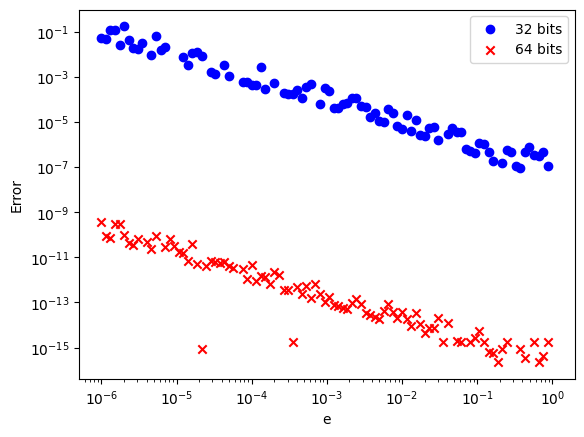
\includegraphics[scale=0.50]{./img/error_numerico_32vs64.png}}
\caption{Error Numérico}
\label{result_errorNumerico}
\end{figure}

Como podemos observar, el error numérico se encuentra delimitado con tope inferior y superior para cada $\epsilon$ y a menores $\epsilon$ el error numérico en la solución es mas grande y decrece a medida que aumenta $\epsilon$. De la misma forma, el error numérico para 64 bits es varios ordenes de magnitud más chico que para 32 bits, ya que se aumenta la precisión en los cálculos.



\subsection{Verificación de la implementación}
Para probar nuestra implementación de sistema tridiagonal se nos pidió resolver una serie de ecuaciones diferenciales. Debemos encontrar \textit{u} para el problema $\frac{\partial^2}{\partial x^2}u = d$ utilizando la matriz tridiagonal del operador laplaciano.
Como mencionamos anteriormente (sección \ref{Intro_laplaciano}), para el caso unidimensional la operación discreta de $\frac{\partial^2}{\partial x^2}u = d$ está dada por:

u$_{i-1}$ - 2u$_{i}$ + u$_{i+1}$ = d$_{i}$

Esta ecuación forma un sistema matricial como se muestra en la figura \ref{laplaciano}. Esta matriz es tridiagonal y siguiendo la estructura de la matriz de la sección \ref{tridiagonal} toma valores:

\begin{itemize}
    \item a: vector de valores 1.
    \item b: vector de valores -2.
    \item c: vector de valores 1.
\end{itemize}

\begin{figure}[H]
    \[ \begin{bmatrix}
-2 & 1 & & & 0\\
1 & -2 & 1 & & & \\
    & 1 & -2 & \ddots & \\
    &    & \ddots &  \ddots & 1\\
0   &    &   & 1 & -2
     \end{bmatrix}
     \begin{bmatrix}
           u_{1}\\
           u_{2} \\
           u_{3}\\ 
           \vdots\\ 
           u_{n}  
     \end{bmatrix}
      =
     \begin{bmatrix}
          d_{1} \\
          d_{2}\\
          d_{3}\\
         \vdots\\ 
         d_{n}  
     \end{bmatrix} \]
     \caption{Forma matricial}\label{laplaciano}
\end{figure}
Por esta estructura,  el algoritmo de eliminación gaussiana para tridiagonales puede aplicarse eficientemente resolviendo el sistema de ecuaciones resultantes de la discretización. Además, como la matriz es diagonal dominante, no es necesario el pivoteo pues no hay riesgo de división por cero. 

De esta forma, se modelaron los tres vectores $d$ a los cuales nombramos como d$\_vect\_a$, d$\_vec\_b$  y d$\_vec\_c$, que representan las ecuaciones requeridas que se pueden ver a continuación con parámetro $n=101$  y se calcularon las segundas derivadas para los tres casos utilizando el algoritmo que se encuentra en la sección \ref{tridiagonal}.

\begin{enumerate}[label=\alph*)] % (a), (b), (c), ...
\label{ec_ej4}
\item d$_{i}$ = 
    $\begin{cases}
      0\\
      \frac{4}{n} & i=\lfloor \frac{n}{2} \rfloor   +1
    \end{cases}$

\item d$_{i}$ = $\frac{4}{n^{2}}$

\item d$_{i}$ = $\frac{-1+2i}{(n-1)}\frac{12}{n^{2}}$

\end{enumerate}


Con estos resultados, se creó un único gráfico que se muestra en la siguiente Figura \ref{result_laplaciano} obteniendo el resultado esperado.

\begin{figure}[H]
\centerline{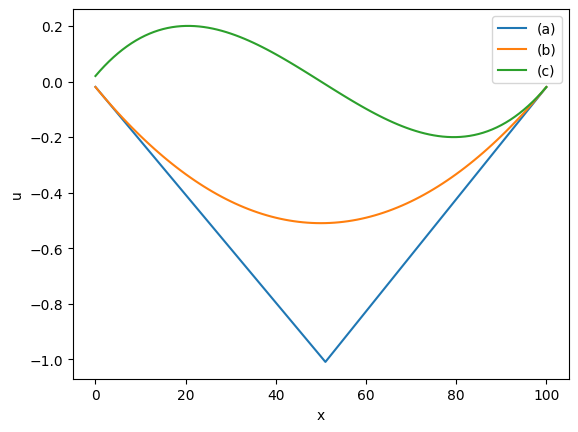
\includegraphics[scale=0.45]{./img/resultado_tridiag}}
\caption{Resultado de las funciones}
\label{result_laplaciano}
\end{figure}

Analizando con mayor profundidad cada función:\par
\begin{enumerate}
    \item[a)] La derivada segunda de la función (a) es 0 para todo x distinto a $i = n/2 + 1$. Luego, la derivada primera de la función (a) es constante para todo x $\not =$ i,lo que implica que la función es lineal para todo x $\not =$ i. Por lo que i es un punto de inflexión. Como la derivada segunda en i es positiva, la función tiene que ser cóncava para los positivos. Esta función descripta es coherente con la figura graficada.

    \item[b)] La derivada segunda de la función (b) es $\frac{4}{n^2}$ para todo x. Entonces, la derivada primera es lineal para todo x, lo que implica que la función es cuadrática para todo x. La función graficada se corresponde con una cuadrática.

    \item[c)] La derivada segunda de la función (c) es una función lineal para todo x. Esto significa que la derivada primera es cuadrática, implicando que la función debe ser un polinomio de grado tres (cúbica). La función graficada se corresponde con una cúbica.
\end{enumerate}



\subsection{Tiempos de cómputo}
Como explicamos anteriormente, los diferentes algoritmos tienen complejidades computacionales muy distintas, lo que afecta significativamente el tiempo de ejecución y los recursos necesarios para resolver un problema.

En el caso de la eliminación gaussiana, el algoritmo con pivoteo tiene una complejidad cúbica ($\mathcal{O}$(n$^3$)), lo que significa que el tiempo de ejecución crece rápidamente a medida que aumenta el tamaño de la matriz. Por otro lado, los algoritmos diseñados específicamente para matrices con estructura especial, como el caso de las matrices tridiagonales, pueden reducir esa complejidad a $\mathcal{O}$(n), lo que implica una mejora considerable en términos de rendimiento.Por lo tanto, Lo esperado es que el algoritmo tridiagonal sea notablemente más rápido a comparación del algoritmo de eliminación gaussiana con pivoteo

Para evaluar el rendimiento de los distintos algoritmos de eliminación gaussiana, se generaron matrices y vectores correspondientes a cada tamaño seleccionado. Posteriormente, se implementaron los algoritmos de eliminación gaussiana con pivoteo, eliminación gaussiana para matrices tridiagonales, tanto en su versión estándar como en la versión con precomputo, para dimensiones que corresponden a potencias de dos (2$^k$). Este proceso fue repetido 10 veces, registrando el tiempo mínimo de ejecución en cada iteración. Esta repetición busca mitigar el posible efecto de las variaciones causadas por la organización del computador (posición de las variables en memoria por ejemplo).

Considerando, las complejidades temporales teóricas de los algoritmos:

\begin{itemize}
    \item Eliminación Gaussiana con pivoteo: $O(n^{3})$
    \item Eliminación Gaussiana para matrices tridiagonales estándar: $O(n)$
    \item Eliminación Gaussiana para matrices tridiagonales con precomputo: $O(n)$
\end{itemize}


Definimos \textit{A} como la matriz Laplaciana, es decir, aquella matriz que tiene a -2 como elementos de la diagonal y a 1 como los elementos de las dos subdiagonales. Obtenemos el siguiente resultado (figura \ref{result_ej5})

\begin{figure}[H]
\centerline{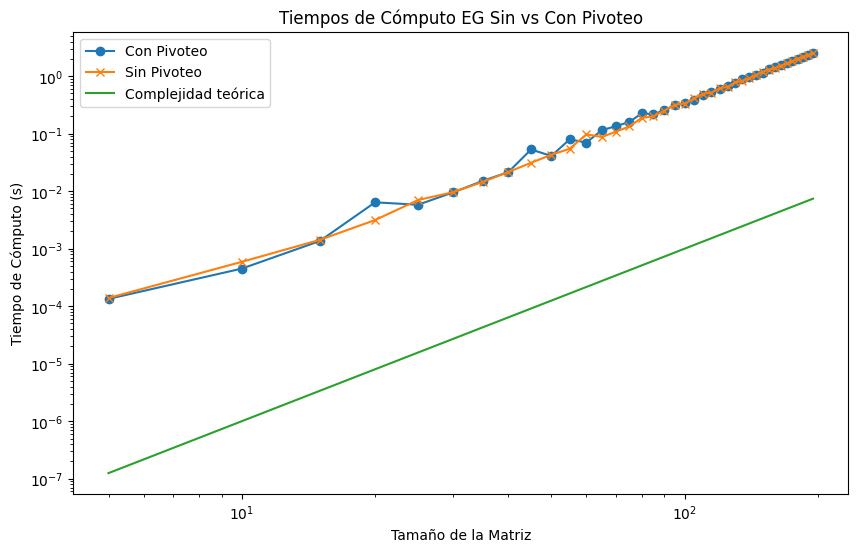
\includegraphics[scale=0.45]{./img/tiempos_EGsinVsConPivoteo.png}}
\caption{Tiempo de computo para EG con pivoteo y EG en un sistema tridiagonal}
\label{result_ej5}
\end{figure}

Como era esperado, como los algoritmos de las matrices tridiagonales trabajan a nivel vectorial, modificando los valores de los vectores b y c, la complejidad temporal mejora.

Por otro lado, realizamos la comparación entre la implementación de EG para un sistema tridiagonal y su variante con precómputo. En la figura \ref{result_ej5_2do} podemos observar claramente el beneficio en el tiempo de ejecución al utilizar la segunda variante del algoritmo, especialmente cuando la cantidad de sistemas a resolver es crecientemente superior a la dimensión del sistema.

\begin{figure}[H]
\centerline{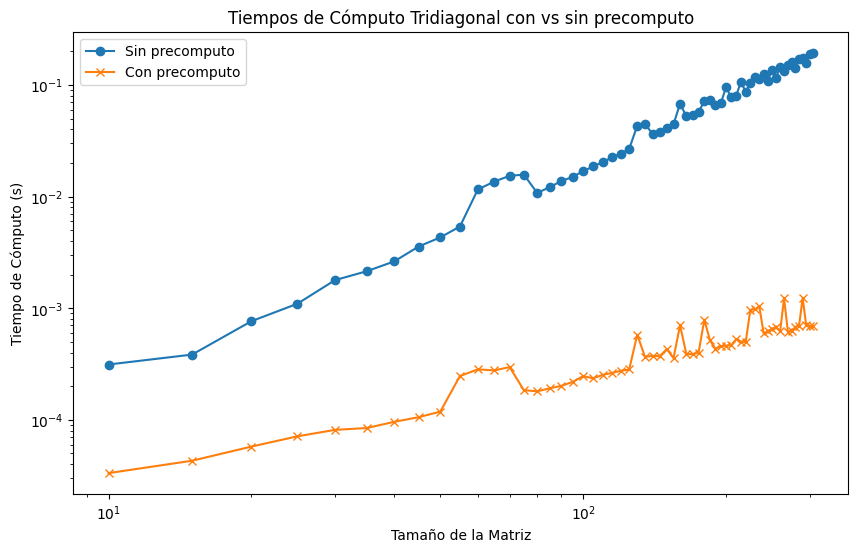
\includegraphics[scale=0.45]{./img/tiempos_tridiagConVsSinP.png}}
\caption{Tiempo de computo para Eliminación Gaussiana tridiagonal estandar vs. precomputada}
\label{result_ej5_2do}
\end{figure}

%Los resultados obtenidos se pueden ver en la sección \ref{resultados}


\subsection{Simulación de difusión}

Para expresar la ecuación de difusión se considera el incremento para el paso \textit{k}, $u^k - u^{k-1}$ como una
fracción ($\alpha$) del operador laplaciano aplicado a $u^{k-1}$ (ecuación explícita) y a $u^{k}$ (ecuación implícita):
\begin{center}
  $u_i^{(k)} - u_i^{(k-1)}$ = $\alpha(u_{i-1}^{(k-1)} - 2u_i^{(k-1)} + u_{i+1}^{(k-1)}) - Eq (3)$
\end{center}

\begin{center}
  $u_i^{(k)} - u_i^{(k-1)}$ = $\alpha(u_{i-1}^{(k)} - 2u_i^{(k)} + u_{i+1}^{(k)}) - Eq (4)$
\end{center}

Reordenando los términos, obtenemos una solución de forma explícita para la ecuación (3). Ésta responde a la forma $u^{(k)} = A \times u^{(k-1)}$. Por otro lado, reordenando los términos de la ecuación (4) obtenemos una solución de forma implícita: A$\times u^{(k)}$ = $u^{(k-1)}$. De esta forma, para obtener la evolución, resolvemos el sistema de ecuaciones para cada paso $k$.

Dada la ecuación:

\begin{equation}
u_{i}^{(k)} - u_{i}^{(k-1)} = \alpha \times (u_{i-1}^{(k)} - 2u_{i}^{(k)} + u_{i+1}^{(k)})
\end{equation}

Se observa que la siguiente ecuación es la ecuación anterior expresada en forma matricial:

\begin{equation}
(I - \alpha \times H) \times u^{(k)} = u^{(k-1)}
\end{equation}

donde:

\begin{itemize}
  \item u$^{(j)}$: vector u en el paso j de difusión
  \item H: matriz Laplaciana de n $\times$ n
  \item I: matriz Identidad de n $\times$ n
\end{itemize}

Demostración:

\begin{equation}
u_{i}^{(k)} - u_{i}^{(k-1)} = \alpha \times (u_{i-1}^{(k)} - 2u_{i}^{(k)} + u_{i+1}^{(k)}) \space \forall i \in [1, n]
\end{equation}

\begin{equation}
\begin{bmatrix}
u_{1}\\
...\\
u_{n}
\end{bmatrix}^{(k)}
-
\begin{bmatrix}
u_{1}\\
...\\
u_{n}
\end{bmatrix}^{(k-1)}
=
\alpha \times H \times
\begin{bmatrix}
u_{1}\\
...\\
u_{n}
\end{bmatrix}^{(k)}
\end{equation}

\begin{equation}
u^{(k)} - u^{(k-1)} = \alpha \times H \times u^{(k)}
\end{equation}

\begin{equation}
u^{(k)} - \alpha \times H \times u^{(k)} =  u^{(k-1)}
\end{equation}

\begin{equation}
(I - \alpha H) \times u^{(k)} = A \times u^{(k)} =  u^{(k-1)}
\end{equation}

Consecuentemente, A = I - $\alpha \times$ H.


Utilizando la última formulación, logramos generar soluciones estables para todos los valores.

Para la solución implícita podemos notar que se genera un sistema tridiagonal, lo que nos permite utilizar el algoritmo de eliminación Gaussiana para sistemas tridiagonales. La eliminación Gaussiana no requiere pivoteo por la estructura de la matriz de derivada segunda. La triangulación finaliza en una matriz donde los elementos de la diagonal principal son: $a_{ii} = - \frac{i+1}{i}$. 
Es así que, como en ningún paso queda un elemento de la diagonal igual a cero, no se requiere pivoteo.\par

Para investigar los distintos grados de difusión utilizamos lso parámetros n = 101, r = 10, m = 1000 y ajustamos el parámetro $\alpha$, el cual se considera como una medida de la tasa de difusión en un modelo específico. Este valor representa una fracción del operador laplaciano, el cual interviene directamente en el cálculo de la difusión de un paso discreto al siguiente.
Al modificar $\alpha$, se observa cómo varía el patrón y la velocidad de difusión de la entidad en cuestión. Por ejemplo, la primer experimentación que se realizo se tomó $\alpha$ = 1 obteniendo el resultado que se muestra en la figura \ref{result_dif}. Se pudo observar que el gráfico obtenido es equivalente al brindado por la cátedra.

A partir de esto, se planteo que a partir de valores más altos de $\alpha$, la difusión sería mayor, siendo probable que veamos una difusión más rápida, donde la entidad se propaga más lejos desde su punto de origen en un período de tiempo determinado.
Mientras que con valores más bajos de $\alpha$, la difusión sería menor siendo probable que la difusión sea más lenta y limitada en alcance.
Para realizar al experimentación, se crearon los vectores con los mismos datos para $\alpha$ = 1, variando únicamente este ultimo parámetro al cual se le asigno valores de 0.1, 0.5 y 2.
A continuación, se generaron los cuatro gráficos que se pueden observar en las figuras \ref{fig:awesome_image1}, \ref{dif0.5} y \ref{fig:awesome_image2}.
%\begin{figure}[htbp]
%\centerline{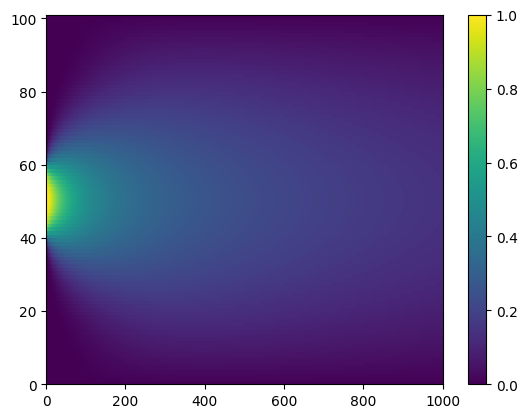
\includegraphics[scale=0.45]{./img/result_dif.png}}
%\caption{Resultado difusión para $\alpha$ = 1}
%\label{result_dif}
%\end{figure}

\begin{figure}[H] 
  \label{ fig7} 
  \begin{minipage}[b]{0.5\linewidth}
    \centering
    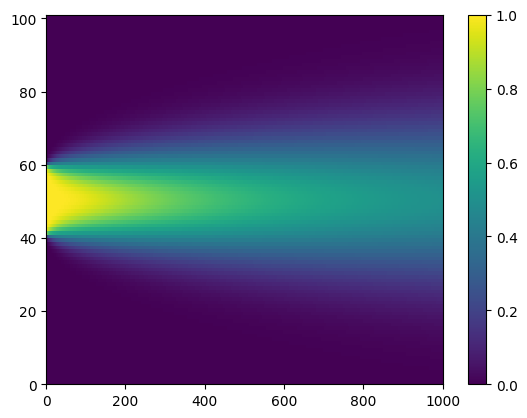
\includegraphics[width=.5\linewidth]{./img/alfa1.png}
  \caption{Difusión $\alpha$ = 0.1}\label{fig:awesome_image1} 
    \vspace{4ex}
  \end{minipage}%%
  \begin{minipage}[b]{0.5\linewidth}
      \centering
    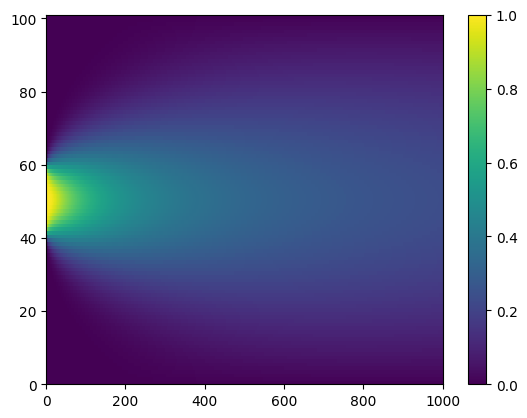
\includegraphics[width=.5\linewidth]{./img/alfa05.png} 
    \caption{Difusión $\alpha$ = 0.5} \label{dif0.5} 
    \vspace{4ex}
  \end{minipage} 
  \begin{minipage}[b]{0.5\linewidth}
    \centering
    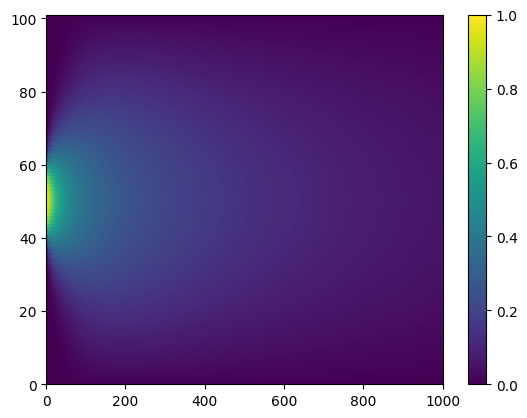
\includegraphics[width=.5\linewidth]{./img/alfa2.png}
  \caption{Difusion $\alpha$ = 2}\label{fig:awesome_image2}
    \vspace{4ex}
  \end{minipage}%% 
  \begin{minipage}[b]{0.5\linewidth}
    \centering
    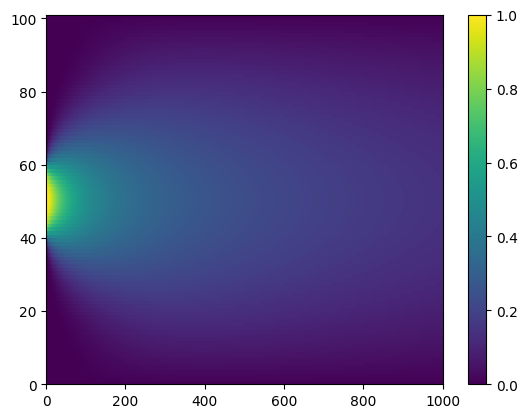
\includegraphics[width=.5\linewidth]{./img/result_dif.png}
  \caption{Difusión $\alpha$ = 1}\label{result_dif}
    \vspace{4ex}
  \end{minipage} 
\end{figure}








\subsubsection{Simulación de difusión 2D}

Al implementar la simulación de la difusión de calor en una placa de 15x15 unidades, se considera una fuente de calor en el punto central con una temperatura constante de 100 unidades, mientras que los bordes de la placa permanecen a 0 en todo momento. Esta simulación, basada en el método implícito, se rige por la ecuación de difusión, que modela cómo el calor se propaga a lo largo del tiempo.
 Como utilizaremos el método implícito, cada paso de tiempo requiere resolver un sistema de ecuaciones lineales. Esto nos garantiza estabilidad, incluso si el coeficiente de difusión $\alpha$ = 0.1 varía.
Por otro lado, a diferencia de la simulación anterior la matriz resultante en 2D no será tridiagonal, sino pentadiagonal, debido a que cada punto de la placa interactúa con sus vecinos en las cuatro direcciones.
En la figura \ref{result_dif} podemos visualizar cómo cambia la distribución de temperatura en la placa a medida que pasa el tiempo.

\begin{figure}[H]
\centerline{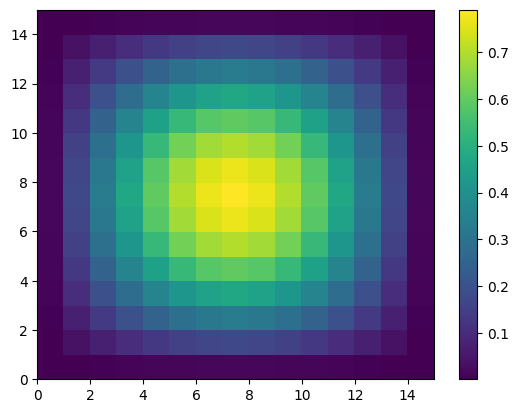
\includegraphics[scale=0.45]{./img/2Dcasoborde0.png}}
\caption{Resultado simulación de difusión de calor en una placa 2D, condiciones de borde con temperatura 0}
\label{result_dif}
\end{figure}



Realizando la comparación de los tiempos de cómputo para la resolución del sistema de ecuaciones de difusión de calor en 2D utilizando los métodos vistos anteriormente (eliminación gaussiana con y sin pivoteo) pudimos observar en la figura \ref{tiempos_dif2D} que, como era de esperar, el tiempo de cómputo aumenta de manera rápida a medida que el tamaño de la matriz crece. Esto se relaciona con el número de operaciones realizadas para resolver el sist. de ec. lineales ya que ésta crece aproximadamente de manera cúbica con el tamaño de la matriz.
Para matrices pequeñas (hasta tamaño 10x10), el tiempo de cómputo es prácticamente el mismo por lo que sugiere que el pivote no añade un costo computacional significativo. Sin embargo, para matrices más grandes (12x12 en adelante), se empieza a notar una diferencia pues el pivoteo mejora la estabilidad numérica del sistema.

\begin{figure}[H]
\centerline{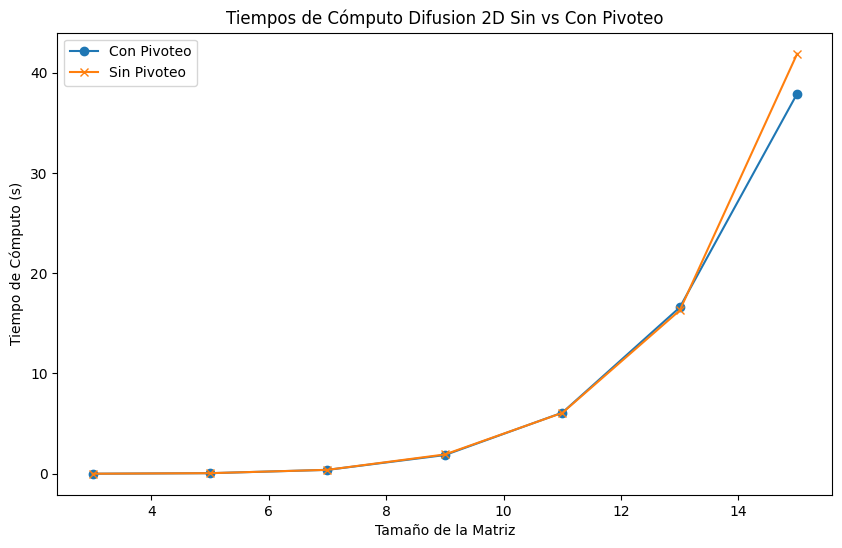
\includegraphics[scale=0.45]{./img/Dif2D_tiempos.png}}
\caption{ Tiempos de cómputo para la resolución del sistema de ecuaciones de difusión de calor en 2D}
\label{tiempos_dif2D}
\end{figure}



Dado que los bordes tienen una temperatura fija de 0, el calor tenderá a disiparse hacia estos, lo que limitará su propagación.
Podemos observar que en el instante t=10 en la figura \ref{instante10}, el calor ya comenzó a propagarse significativamente desde el centro, pero todavía no ha llegado a los bordes de la placa, lo que es esperable porque aún estamos en un tiempo relativamente temprano en la simulación. A su vez, la distribución suave de la temperatura en los alrededores de la fuente central sugiere que el método implícito utilizado está funcionando bien, ya que evita oscilaciones o comportamientos inestables.



\begin{figure}[H] 
  \label{ fig7} 
  \begin{minipage}[b]{0.5\linewidth}
    \centering
    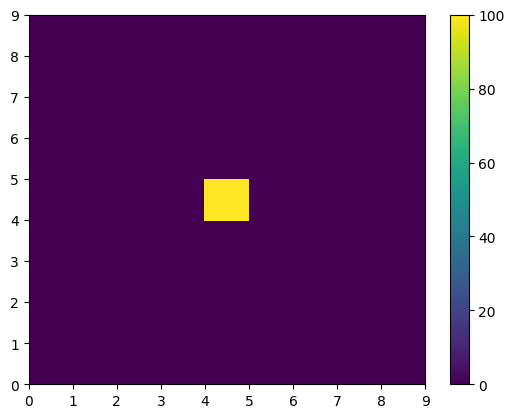
\includegraphics[width=.5\linewidth]{./img/instante0.png}
  \caption{Difusión $\alpha$ = 0.1}\label{instante0} 
    \vspace{4ex}
  \end{minipage}%%
  \begin{minipage}[b]{0.5\linewidth}
      \centering
    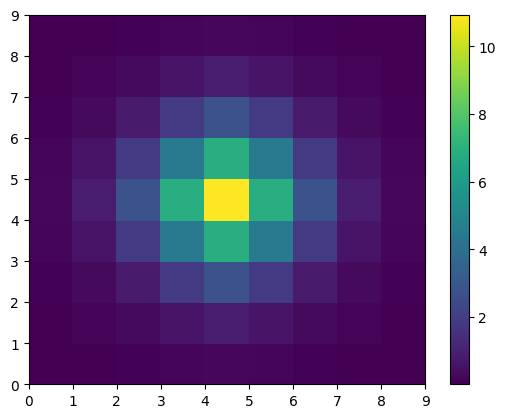
\includegraphics[width=.5\linewidth]{./img/instante10.png} 
    \caption{Instante $t$ = 10} \label{instante10} 
    \vspace{4ex}
  \end{minipage} 
  \begin{minipage}[b]{0.5\linewidth}
    \centering
    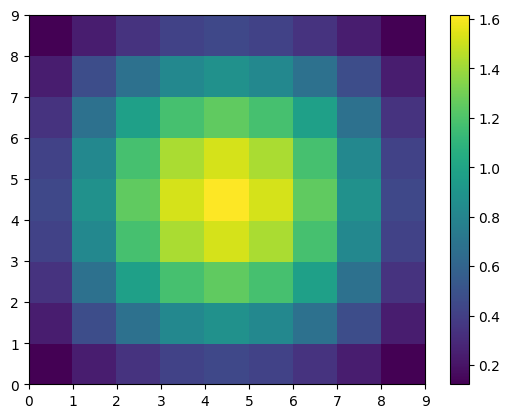
\includegraphics[width=.5\linewidth]{./img/instante50.png}
  \caption{Instante $t$ = 50}\label{instante50}
    \vspace{4ex}
  \end{minipage}%% 
  \begin{minipage}[b]{0.5\linewidth}
    \centering
    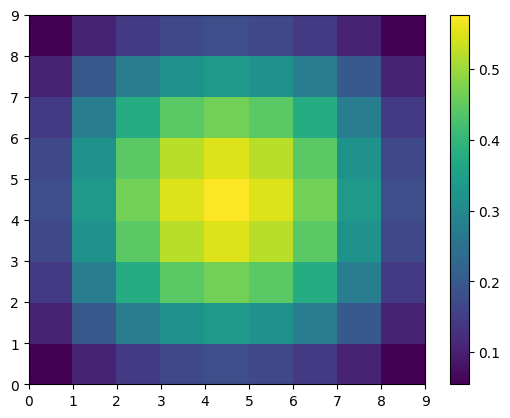
\includegraphics[width=.5\linewidth]{./img/instante100.png}
  \caption{Instante $t$ = 100}\label{instante100}
    \vspace{4ex}
  \end{minipage} 
\end{figure}






\iffalse
    \subsection{Resultado de eliminación Gaussiana sin pivoteo}
    \label{resultados EG}

    \subsubsection{Ejercicio 1.1}
    El pseudocódigo de la función implementada se puede encontrar en la sección \ref{EG_sinP}

    \subsubsection{Ejercicio 1.2}

    Ya est´á dentro de la introducci´ón.



    Si tomamos de ejemplo a la siguiente matriz:

    \begin{center}
    $\begin{bmatrix}
    0 & 1 & -1 & 3\\
    -2 & -0.5 & 0 & 0\\
    4 & 1 & -2 & 4\\
    -6 & -1 & 2 & -3
    \end{bmatrix}$
    \end{center}
                  
    Es esperado que al procesarla se produzca un error debido a que para resolver el sistema necesitamos intercambiar filas y columnas para llevar la matriz a una forma triangular superior y el algoritmo no lo realiza, pues solo se permite operaciones de multiplicación y suma para reducir los elementos debajo de la diagonal principal.

    \subsection{Resultado de eliminación Gaussiana con pivoteo}
    \label{resultados EG c/p}
    \subsubsection{Ejercicio 2.1}
    El pseudocódigo de la función implementada se puede encontrar en la sección \ref{seccion_EG_pivot}

    \subsubsection{Ejercicio 2.2}

Movido a la introducción

\fi




\iffalse
    \subsection{Ejercicio 2.3}

    Se tiene el sistema de ecuaciones lineales con A y b igual a:

    \[ \begin{bmatrix}  
    1 & 2+\epsilon & 3-\epsilon\\
    1-\epsilon & 2 & 3+\epsilon\\
    1+\epsilon & 2-\epsilon & 3
    \end{bmatrix} ,
    \begin{bmatrix}
    6\\
    6\\
    6
    \end{bmatrix}\]
    
    Se calcula la matriz inversa de A, $A^{-1}$:    
    \begin{center}
    $\begin{bmatrix}
    \frac{\epsilon+1}{18\epsilon} & \frac{\epsilon-8}{18\epsilon} & \frac{\epsilon+7}{18\epsilon}\\
    \frac{\epsilon+7}{18\epsilon} & \frac{\epsilon-2}{18\epsilon} & \frac{\epsilon-5}{18\epsilon}\\
    \frac{\epsilon-5}{18\epsilon} & \frac{\epsilon+4}{18\epsilon} & \frac{\epsilon+1}{18\epsilon}
    \end{bmatrix}$
    \end{center}

    Con este resultado es sencillo notar que el único $\epsilon$ que genera que A no tenga inversa es 0. Para el resto, A tiene inversa y por lo tanto el sistema de ecuaciones tiene una única solución. Cuando multiplicamos a $A^{-1}$ por b, obtenemos que el vector solución es x$^t$ = [1, 1, 1], independientemente del $\epsilon$. Por lo tanto, la solución del algoritmo de pivoteo parcial debería devolver siempre x$^t$ = [1, 1, 1]. Sin embargo, se espera que por error numérico esto no sea así. 

    La norma infinito de $A$ es 6 y la de $A^{-1}$ es $\frac{\epsilon+16}{18\epsilon}$. Por lo tanto el numero de condición para $A$ es $\frac{\epsilon+16}{3\epsilon}$. Si $\epsilon$ tiende a cero, el numero de condición para $A$ es infinito. Si en cambio, tiende a infinito, el numero de condición es 1/3. Entonces, cuanto más grande es $\epsilon$, más chico es el numero de condición y más estable es A. 

    El gráfico a continuación muestra la comparación entre el error absoluto vs $\epsilon$ para variables de 32 bits y 64 bits:

    \begin{figure}[htbp]
    \centerline{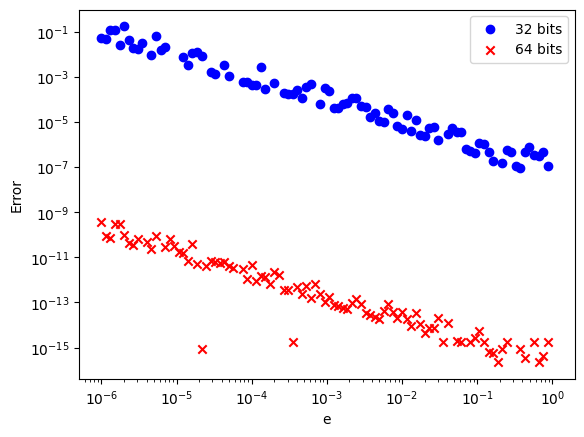
\includegraphics[scale=0.50]{./img/error_numerico_32vs64.png}}
    \caption{Error Numérico}
    \label{result_errorNumerico}
    \end{figure}

    Como podemos observar, el error numérico se encuentra delimitado con tope inferior y superior para cada $\epsilon$ y a menores $\epsilon$ el error numérico en la solución es mas grande y decrece a medida que aumenta $\epsilon$. De la misma forma, el error numérico para 64 bits es varios ordenes de magnitud más chico que para 32 bits, ya que se aumenta la precisión en los cálculos.

\fi


%%%%%%%%%%%%%%%%%%%%%%%%%%%%%%
\iffalse
    \subsection{Resultado Verificación de la implementación}
    \label{resultados derivada}
    Realizamos el cálculo de la derivada segunda de manera discreta para las tres funciones especificadas por la cátedra utilizando la implementación de eliminación Gaussiana para un sistema tridiagonal.
    Se generaron los vectores d$\_vect\_a$, d$\_vec\_b$  y d$\_vec\_c$ que representan las funciones que se encuentran en la sección \ref{tridiagonal} y se calcularon las segundas derivadas para los tres casos.
    Con estos resultados, se creó un único gráfico que se muestra en la siguiente Figura \ref{result_laplaciano} obteniendo el resultado esperado.

    \begin{figure}[H]
    \centerline{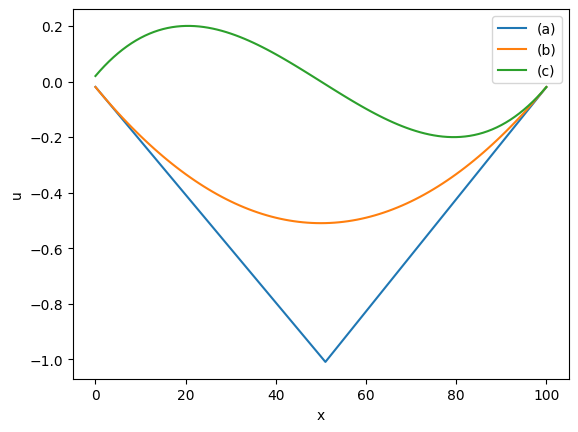
\includegraphics[scale=0.45]{./img/resultado_tridiag}}
    \caption{Resultado de las funciones}
    \label{result_laplaciano}
    \end{figure}

    Analizando con mayor profundidad cada función:\par
    \begin{enumerate}
        \item[a)] La derivada segunda de la función (a) es 0 para todo x distinto a $i = n/2 + 1$. Luego, la derivada primera de la función (a) es constante para todo x $\not =$ i,lo que implica que la función es lineal para todo x $\not =$ i. Por lo que i es un punto de inflexión. Como la derivada segunda en i es positiva, la función tiene que ser cóncava para los positivos. Esta función descripta es coherente con la figura graficada.

        \item[b)] La derivada segunda de la función (b) es $\frac{4}{n^2}$ para todo x. Entonces, la derivada primera es lineal para todo x, lo que implica que la función es cuadrática para todo x. La función graficada se corresponde con una cuadrática.

      \item[c)] La derivada segunda de la función (c) es una función lineal para todo x. Esto significa que la derivada primera es cuadrática, implicando que la función debe ser un polinomio de grado tres (cúbica). La función graficada se corresponde con una cúbica.
    \end{enumerate}
\fi    
    
%%%%%%%%%%%%%%%%%%%%%%%%%%%%%%
    
    

\iffalse
    \subsection{Resultado Tiempos de cómputo}
    \label{resultados tiempo}
    \subsubsection{Ejercicio 5.1}
    El objetivo de este ejercicio es obtener de forma experimental la complejidad temporal de los algoritmos utilizados en los puntos anteriores: eliminación Gaussiana con pivoteo, eliminación Gaussiana para matrices tridiagonales estándar y con precomputo. Las complejidades temporales teóricas de los algoritmos son:

    \begin{itemize}
        \item Eliminación Gaussiana con pivoteo: $O(n^{3})$
        \item Eliminación Gaussiana para matrices tridiagonales estándar: $O(n)$
        \item Eliminación Gaussiana para matrices tridiagonales con precomputo: $O(n)$
    \end{itemize}

    El algoritmo de Eliminación Gaussiana con pivoteo tiene un triple for, necesario para la triangulación de la matriz A. Lo que genera que la complejidad temporal sea cúbica. En cambio los algoritmos de las matrices tridiagonales trabajan a nivel vectorial, modificando los valores de los vectores b y c. Lo que genera que la complejidad temporal sea lineal.

    Para este ejercicio se definió \textit{A} como la matriz Laplaciana, es decir, aquella matriz que tiene a -2 como elementos de la diagonal y a 1 como los elementos de las dos subdiagonales.

    \begin{figure}[H]
    \centerline{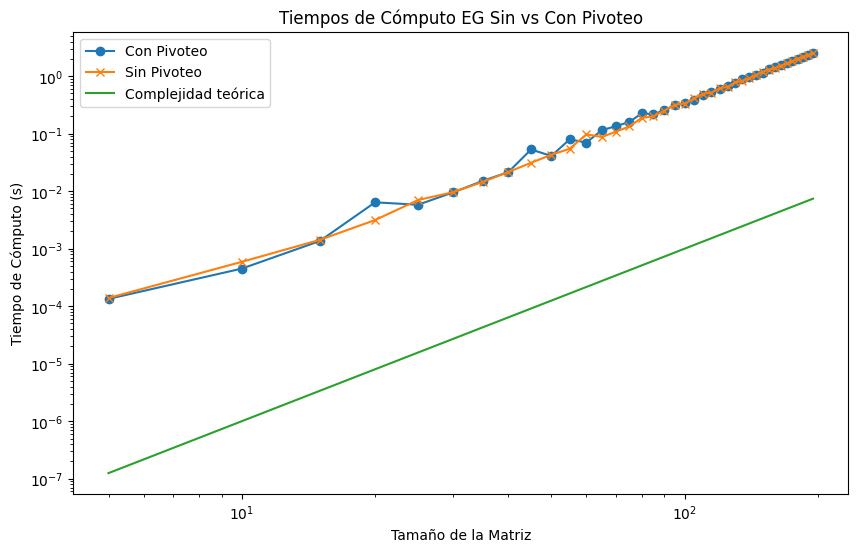
\includegraphics[scale=0.45]{./img/tiempos_EGsinVsConPivoteo.png}}
    \caption{Tiempo de computo para EG con pivoteo y EG en un sistema tridiagonal}
    \label{result_ej5}
    \end{figure}
\fi

%%%%%%%%%%%%%%%%%%%%%%%%%%%%%%

\iffalse
    \subsubsection{Ejercicio 5.2}

    Con el resultado obtenido, se ve claramente el beneficio en el tiempo de ejecución al utilizar la segunda variante del algoritmo, especialmente cuando la cantidad de sistemas a resolver es crecientemente superior a la dimensión del sistema.

    \begin{figure}[H]
    \centerline{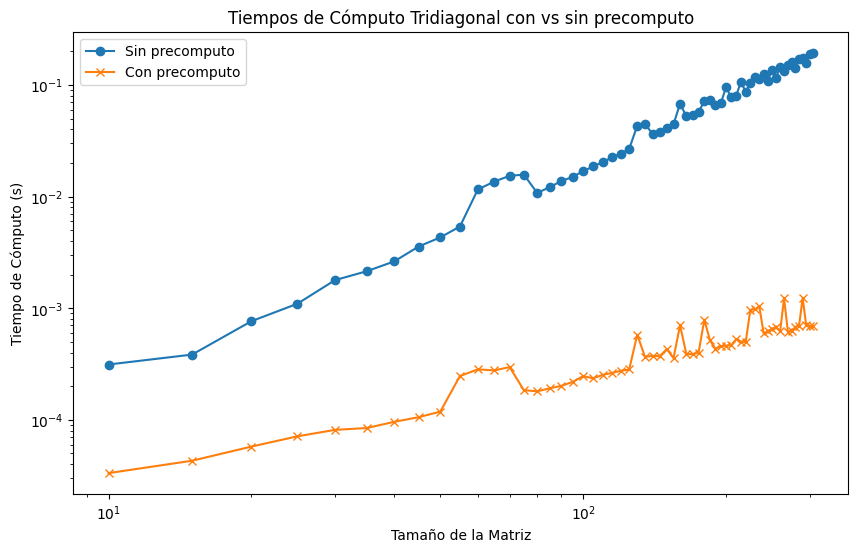
\includegraphics[scale=0.45]{./img/tiempos_tridiagConVsSinP.png}}
    \caption{Tiempo de computo para Eliminación Gaussiana tridiagonal estandar vs. precomputada}
    \label{result_ej5_2do}
    \end{figure}

\fi

%%%%%%%%%%%%%%%%%%%%%%%%%%%%%%
\iffalse
    \subsection{Resultado Difusión}
    \label{difusion}
    \subsubsection{Ejercicio 6.1}
    Dada la ecuación:
    
    \begin{equation}
    u_{i}^{(k)} - u_{i}^{(k-1)} = \alpha \times (u_{i-1}^{(k)} - 2u_{i}^{(k)} + u_{i+1}^{(k)})
    \end{equation}

    Se observa que la siguiente ecuación es la ecuación anterior expresada en forma matricial:

    \begin{equation}
    (I - \alpha \times H) \times u^{(k)} = u^{(k-1)}
    \end{equation}

    donde:

    \begin{itemize}
      \item u$^{(j)}$: vector u en el paso j de difusión
      \item H: matriz Laplaciana de n $\times$ n
      \item I: matriz Identidad de n $\times$ n
    \end{itemize}

    Demostración:

    \begin{equation}
    u_{i}^{(k)} - u_{i}^{(k-1)} = \alpha \times (u_{i-1}^{(k)} - 2u_{i}^{(k)} + u_{i+1}^{(k)}) \space \forall i \in [1, n]
    \end{equation}

    \begin{equation}
    \begin{bmatrix}
    u_{1}\\
    ...\\
    u_{n}
    \end{bmatrix}^{(k)}
    -
    \begin{bmatrix}
    u_{1}\\
    ...\\
    u_{n}
    \end{bmatrix}^{(k-1)}
    =
    \alpha \times H \times
    \begin{bmatrix}
    u_{1}\\
    ...\\
    u_{n}
    \end{bmatrix}^{(k)}
    \end{equation}
    
    \begin{equation}
    u^{(k)} - u^{(k-1)} = \alpha \times H \times u^{(k)}
    \end{equation}
    
    \begin{equation}
    u^{(k)} - \alpha \times H \times u^{(k)} =  u^{(k-1)}
    \end{equation}
    
    \begin{equation}
    (I - \alpha H) \times u^{(k)} = A \times u^{(k)} =  u^{(k-1)}
    \end{equation}

    Consecuentemente, A = I - $\alpha \times$ H.
\fi

%%%%%%%%%%%%%%%%%%%%%%%%%%%%%%
\iffalse
    \subsubsection{Ejercicio 6.2}
    Para investigar los distintos grados de difusión, ajustamos el parámetro $\alpha$, el cual se considera como una medida de la tasa de difusión en un modelo específico. Este valor representa una fracción del operador laplaciano, el cual interviene directamente en el cálculo de la difusión de un paso discreto al siguiente.
    Al modificar $\alpha$, se observa cómo varía el patrón y la velocidad de difusión de la entidad en cuestión. Por ejemplo, la primer experimentación que se realizo se tomó $\alpha$ = 1 obteniendo el resultado que se muestra en la figura \ref{result_dif}. Se pudo observar que el gráfico obtenido es equivalente al brindado por la cátedra.

    A partir de esto, se planteo que a partir de valores más altos de $\alpha$, la difusión sería mayor, siendo probable que veamos una difusión más rápida, donde la entidad se propaga más lejos desde su punto de origen en un período de tiempo determinado.
    Mientras que con valores más bajos de $\alpha$, la difusión sería menor siendo probable que la difusión sea más lenta y limitada en alcance.
    Para realizar al experimentación, se crearon los vectores con los mismos datos para $\alpha$ = 1, variando únicamente este ultimo parámetro al cual se le asigno valores de 0.1, 0.5 y 2.
    A continuación, se generaron los cuatro gráficos que se pueden observar en las figuras \ref{fig:awesome_image1}, \ref{dif0.5} y \ref{fig:awesome_image2}.
    %\begin{figure}[htbp]
    %\centerline{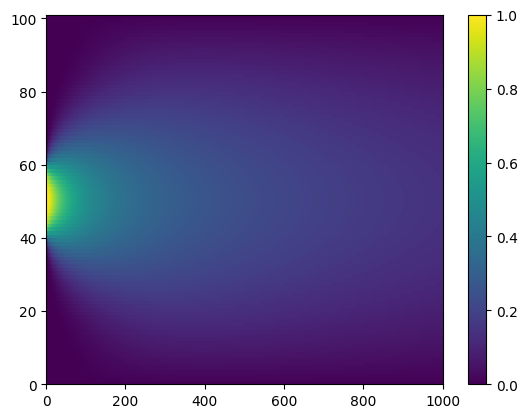
\includegraphics[scale=0.45]{./img/result_dif.png}}
    %\caption{Resultado difusión para $\alpha$ = 1}
    %\label{result_dif}
    %\end{figure}

    \begin{figure}[H] 
      \label{ fig7} 
    \begin{minipage}[b]{0.5\linewidth}
        \centering
        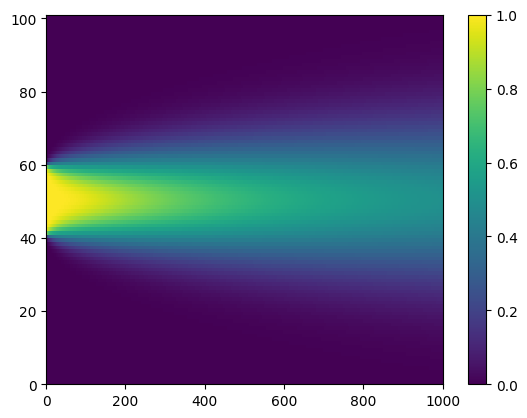
\includegraphics[width=.5\linewidth]{./img/alfa1.png}
      \caption{Difusión $\alpha$ = 0.1}\label{fig:awesome_image1} 
        \vspace{4ex}
      \end{minipage}%%
      \begin{minipage}[b]{0.5\linewidth}
          \centering
        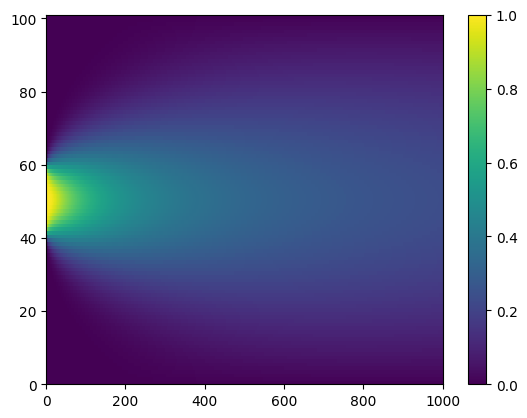
\includegraphics[width=.5\linewidth]{./img/alfa05.png} 
        \caption{Difusión $\alpha$ = 0.5} \label{dif0.5} 
        \vspace{4ex}
      \end{minipage} 
      \begin{minipage}[b]{0.5\linewidth}
        \centering
        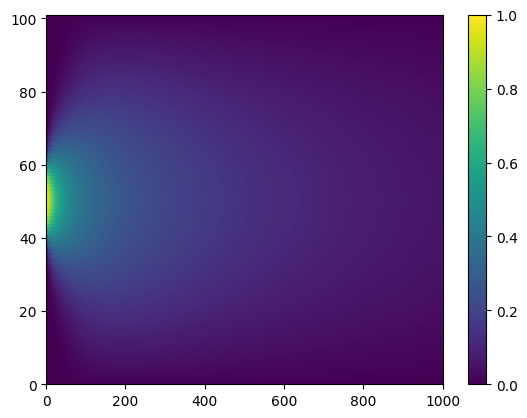
\includegraphics[width=.5\linewidth]{./img/alfa2.png}
      \caption{Difusion $\alpha$ = 2}\label{fig:awesome_image2}
        \vspace{4ex}
      \end{minipage}%% 
      \begin{minipage}[b]{0.5\linewidth}
        \centering
        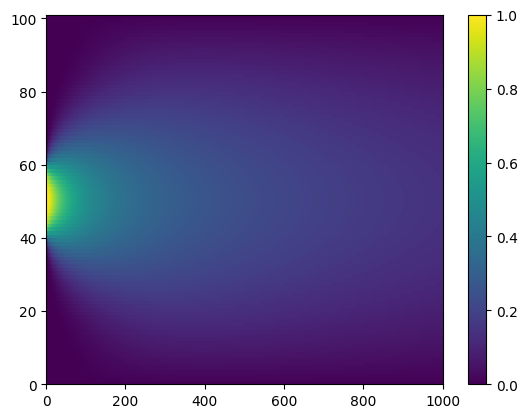
\includegraphics[width=.5\linewidth]{./img/result_dif.png}
      \caption{Difusión $\alpha$ = 1}\label{result_dif}
        \vspace{4ex}
      \end{minipage} 
    \end{figure}
\fi


%%%%%%%%%%%%%%%%%%%%%%%%%%%%%%

\iffalse
    \subsection{Resultado Difusión 2D}
    \label{difusion2D}
    \subsubsection{Ejercicio 7.1}

    \begin{figure}[H]
    \centerline{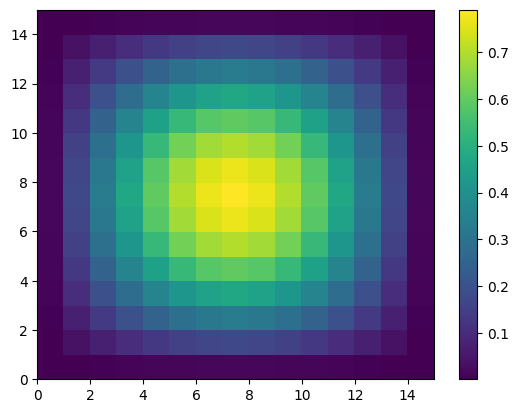
\includegraphics[scale=0.45]{./img/2Dcasoborde0.png}}
    \caption{Resultado simulación de difusión de calor en una placa 2D, condiciones de borde con temperatura 0}
    \label{result_dif}
    \end{figure}

    \subsubsection{Ejercicio 7.2}
    Realizando la comparación de los tiempos de cómputo para la resolución del sistema de ecuaciones de difusión de calor en 2D utilizando los dos métodos vistos anteriormente (eliminación gaussiana con y sin pivoteo) pudimos observar que, como era de esperar, el tiempo de cómputo aumenta de manera rápida a medida que el tamaño de la matriz crece. Esto se relaciona con el número de operaciones realizadas para resolver el sist. de ec. lineales ya que ésta crece aproximadamente de manera cúbica con el tamaño de la matriz.
    Para matrices pequeñas (hasta tamaño 10x10), el tiempo de cómputo es prácticamente el mismo por lo que sugiere que el pivote no añade un costo computacional significativo. Sin embargo, para matrices más grandes (12x12 en adelante), se empieza a notar una diferencia pues el pivoteo mejora la estabilidad numérica del sistema.

    \begin{figure}[H]
    \centerline{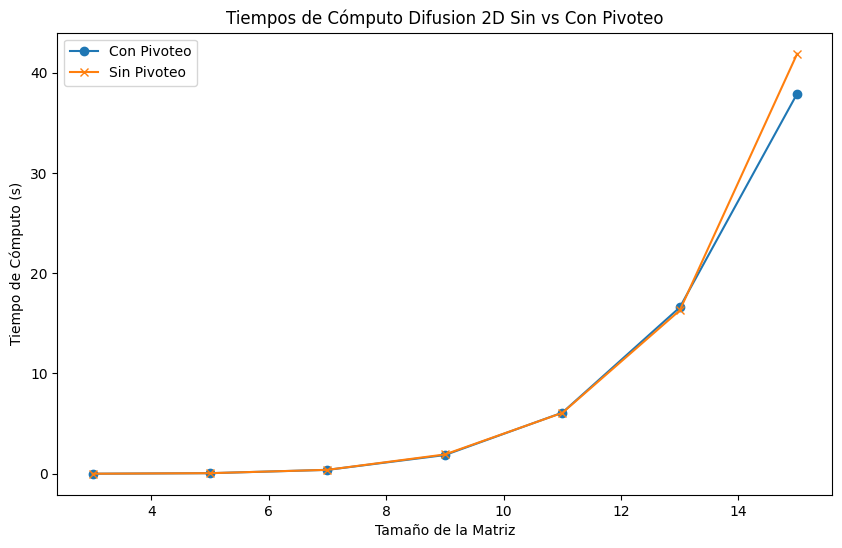
\includegraphics[scale=0.45]{./img/Dif2D_tiempos.png}}
    \caption{ Tiempos de cómputo para la resolución del sistema de ecuaciones de difusión de calor en 2D}
    \label{tiempos_dif2D}
    \end{figure}


    \subsubsection{Ejercicio 7.3}

    \begin{figure}[H] 
      \label{ fig7} 
      \begin{minipage}[b]{0.5\linewidth}
        \centering
        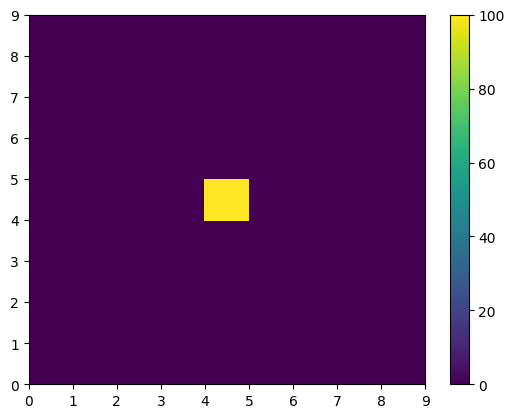
\includegraphics[width=.5\linewidth]{./img/instante0.png}
      \caption{Difusión $\alpha$ = 0.1}\label{instante0} 
        \vspace{4ex}
      \end{minipage}%%
      \begin{minipage}[b]{0.5\linewidth}
         \centering
        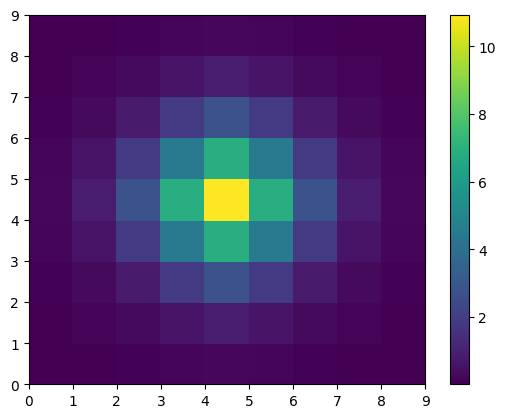
\includegraphics[width=.5\linewidth]{./img/instante10.png} 
        \caption{Instante $t$ = 10} \label{instante10} 
        \vspace{4ex}
      \end{minipage} 
      \begin{minipage}[b]{0.5\linewidth}
        \centering
       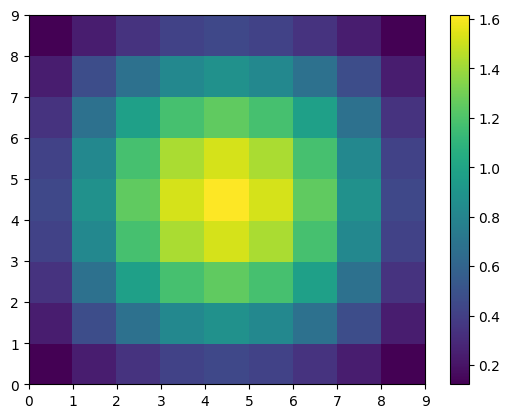
\includegraphics[width=.5\linewidth]{./img/instante50.png}
      \caption{Instante $t$ = 50}\label{instante50}
        \vspace{4ex}
      \end{minipage}%% 
      \begin{minipage}[b]{0.5\linewidth}
       \centering
       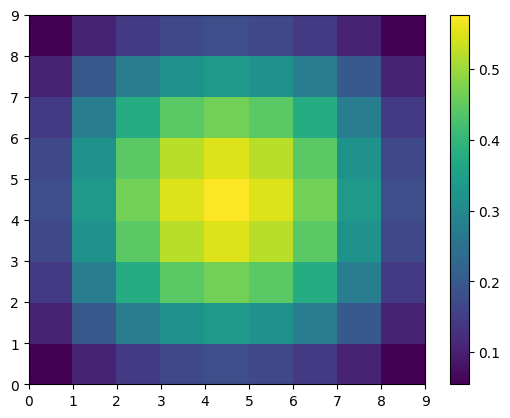
\includegraphics[width=.5\linewidth]{./img/instante100.png}
      \caption{Instante $t$ = 100}\label{instante100}
        \vspace{4ex}
      \end{minipage} 
    \end{figure}


    \subsubsection{Ejercicio 7.4}
    Dado que los bordes tienen una temperatura fija de 0, el calor tenderá a disiparse hacia estos, lo que limitará su propagación.
    Podemos observar que en el instante t=10, el calor ya comenzó a propagarse significativamente desde el centro, pero todavía no ha llegado a los bordes de la placa, lo que es esperable porque aún estamos en un tiempo relativamente temprano en la simulación. A su vez, la distribución suave de la temperatura en los alrededores de la fuente central sugiere que el método implícito utilizado está funcionando bien, ya que evita oscilaciones o comportamientos inestables.
\fi


 \subsection{Opcionales}

 Como mencionamos en la sección \ref{opcionales}, el objetivo es calcular la matriz inversa de una matriz A utilizando el método de eliminación gaussiana (EG) con una matriz aumentada. Para ello se implemento la función \textit{invertir\_sistema} cuyo pseudocódigo es el siguiente: 
 
\begin{algorithm}[H]
\caption{Ejercicio opcional}
\begin{algorithmic}
\State \textbf{EG}(\textbf{in} A : matrix) $\to \textbf{A\_inv}$
 
 \State $n \gets A.shape[0]$
 \State $I \gets matriz\_identidad$
 \State $new\_A \gets eg(A,I)$
 \State $base\_matrix \gets new\_A[0:,:n]$
 \For{$i \gets n$ to $2*n$}
        \State  b $\gets$ new\_A.(1,n)
        \State x $\gets$ resolver$\_$sistema(base$\_$matrix,b)
        \State A$\_$inv[0:,i-n] $\gets$ x
\EndFor

\Return{$A\_inv$}
\end{algorithmic}
\end{algorithm}

Para resolver el problema utilizamos las funciones vistas en el trabajo practico. En la sección \ref{sec:inversa}, mostramos un ejemplo de su aplicación.

\section{Conclusiones}
\label{sec:conclusiones}
\bibliography{bibliography.bib}
\bibliographystyle{plain}
\label{sec:bibliografia}


\iffalse
¿Cómo se usa esto?
-> https://www.youtube.com/watch?v=JwXQb25cpqA&t=3s

¿Cómo encuentro/escribo el formato correcto?
-> https://youtu.be/JwXQb25cpqA?si=mAk9X0Od4TzdwvJ0&t=54

¿Cómo formateo una nueva referencia?
-> https://www.bibtex.org/Format/

¿Cuales son los tipos de referencias y qué campos incluye cada una?
-> https://www.openoffice.org/bibliographic/bibtex-defs.html

\fi


\end{document}
